%%%%%%%%%%%%%%%%%%%%%%%%%%%%%%%%%%%%%%%%%%%%%%%%%%%%%%%%%%
%%%%%%%%%%%%%%%%%%%%%%%%%%%%%%%%%%%%%%%%%%%%%%%%%%%%%%%%%%
%%          Written by Nicolas Bigaouette               %%
%%                    Fall 2012                         %%
%%              nbigaouette@gmail.com                   %%
%%%%%%%%%%%%%%%%%%%%%%%%%%%%%%%%%%%%%%%%%%%%%%%%%%%%%%%%%%
%%%%%%%%%%%%%%%%%%%%%%%%%%%%%%%%%%%%%%%%%%%%%%%%%%%%%%%%%%

\newcommand{\Title}{Computational investigation of intense short-wavelength
                    laser interaction with rare gas clusters}
\newcommand{\Author}{Nicolas Bigaouette}
\newcommand{\AuthorInitials}{NB}

% University of Ottawa thesis formatting
% \documentclass[author={\Author},title={\Title},degree={Ph.D.},linenumbers,draft]{uottawa}
\documentclass[author={\Author},title={\Title},degree={Ph.D.},linenumbers,final]{uottawa}


%%%%%%%%%%%%%%%%%%%%%%%%%%%%%%%%%%%%%%%%%%%%%%%%%%%%%%%
% Useful macros
%%%%%%%%%%%%%%%%%%%%%%%%%%%%%%%%%%%%%%%%%%%%%%%%%%%%%%%
%%%%%%%%%%%%%%%%%%%%%%%%%%%%%%%%%%%%%%%%%%%%%%%%%%%%%%%%%%%%%%%%%%%%%%%%%%%%%%%%%%%%%%
%%%%%%%%%%%%%%%%%%%%%%%%%%%%%%%%%%%%%%%%%%%%%%%%%%%%%%%%%%%%%%%%%%%%%%%%%%%%%%%%%%%%%%
%%                             Usefull macros                                       %%
%%                           Nicolas Bigaouette                                     %%
%%                          nbigaouette@gmail.com                                   %%
%%%%%%%%%%%%%%%%%%%%%%%%%%%%%%%%%%%%%%%%%%%%%%%%%%%%%%%%%%%%%%%%%%%%%%%%%%%%%%%%%%%%%%
%%%%%%%%%%%%%%%%%%%%%%%%%%%%%%%%%%%%%%%%%%%%%%%%%%%%%%%%%%%%%%%%%%%%%%%%%%%%%%%%%%%%%%

% Needed for \onehalf
\usepackage{ltugcomn}
% Needed for bold Greek letters
\usepackage{bm}

\newcommand{\mailto}[1]{\href{mailto:#1}{#1}}

\newcommand{\angstrom}{{\AA}ngstr\"om}

% \newcommand{\vecnabla}{\vec{\nabla}}
\newcommand{\vecnabla}{\bm{\nabla}}
\newcommand{\laplacien}[1]{\vecnabla^2 #1}           % Laplacien
\newcommand{\laplacian}[1]{\laplacien{#1}}           % Laplacien
\newcommand{\laplacient}[1]{\vecnabla_{\bot}^{2} #1} % Laplacien transverse
\newcommand{\gradient}[1]{\vecnabla #1}              % Gradient
\newcommand{\grad}[1]{\vecnabla #1}                  % Gradient
\newcommand{\divergence}[1]{\vecnabla \cdot #1}      % Divergence
\newcommand{\rotationnel}[1]{\vecnabla \times #1}    % Rotationnel

% \newcommand{\spherical}{\ensuremath{\mathcal{Y}}_{l,m}\pa{\theta,\phi}}
%                                                     % Spherical Harmonics Y_lm
\newcommand{\spherical}{Y_{l,m}\pa{\theta,\phi}}         % Spherical Harmonics Y_lm
\newcommand{\sphericalp}{Y_{l,m}\pa{\theta',\phi'}}      % Spherical Harmonics Y_lm
\newcommand{\sphericallmp}{Y_{l',m'}\pa{\theta,\phi}}    % Spherical Harmonics Y_lm
\newcommand{\sphericalpc}{Y_{l,m}^*\pa{\theta',\phi'}}   % Spherical Harmonics Y_lm
\newcommand{\sphericalc}{Y_{l,m}^*\pa{\theta,\phi}}      % Spherical Harmonics Y_lm
\newcommand{\gspherical}{\ensuremath{\mathcal{Y}}_{j,l,m}\pa{\theta,\phi}}
                                                         % Genralized Spherical Harmonics
                                                         % Y_jml

\newcommand{\onehalf}{\sfrac{1}{2}}
\newcommand{\onethird}{\sfrac{1}{3}}
\newcommand{\onefourth}{\sfrac{1}{4}}
\newcommand{\twothird}{\sfrac{2}{3}}
\newcommand{\threehalf}{\sfrac{3}{2}}
\newcommand{\fivehalf}{\sfrac{5}{2}}
\newcommand{\eighthalf}{\sfrac{8}{2}}
\newcommand{\summation}[2]{\sum\limits_{#1}^{#2}}

\newcommand{\im}{\textrm{i}}                                    % i = sqrt{-1}

\newcommand{\mum}{\mu \textrm{m}}                               % mu m

\newcommand{\hbartwo}{\frac{\hbar}{2}}
\newcommand{\twohbar}{\frac{2}{\hbar}}

\newcommand{\dd}[1]{~\textrm{d} #1}

\newcommand{\del}{\partial}                                     % del

\newcommand{\delexp}[3]{\frac{\del^{#3} #1}{\del #2^{#3}}}          % del^? ? / del?
\newcommand{\dexp}[3]{\frac{\textrm{d}^{#3} #1}{\textrm{d} #2^{#3}}}% d^? ? / d?

\newcommand{\delx}[1]{\delexp{#1}{x}{{}}}                     % del ? / delx
\newcommand{\dely}[1]{\delexp{#1}{y}{{}}}                     % del ? / dely
\newcommand{\delz}[1]{\delexp{#1}{z}{{}}}                     % del ? / delz
\newcommand{\delr}[1]{\delexp{#1}{r}{{}}}                     % del ? / delr
\newcommand{\delt}[1]{\delexp{#1}{t}{{}}}                     % del ? / delt
\newcommand{\deli}[2]{\delexp{#1}{{#2}}{{}}}                  % del ? / del?

\newcommand{\delxs}[1]{\delexp{{#1}}{x}{2}}                     % del^2 ? / delx^2
\newcommand{\delys}[1]{\delexp{{#1}}{y}{2}}                     % del^2 ? / dely^2
\newcommand{\delzs}[1]{\delexp{{#1}}{z}{2}}                     % del^2 ? / delz^2
\newcommand{\delts}[1]{\delexp{{#1}}{t}{2}}                     % del^2 ? / delt^2
\newcommand{\delrs}[1]{\delexp{{#1}}{r}{2}}                     % del^2 ? / delr^2
\newcommand{\delis}[2]{\delexp{{#1}}{#2}{2}}                    % del^2 ? / del?^2

\newcommand{\delxt}[1]{\delexp{{#1}}{x}{3}}                     % del^3 ? / delx^3
\newcommand{\delyt}[1]{\delexp{{#1}}{y}{3}}                     % del^3 ? / dely^3
\newcommand{\delzt}[1]{\delexp{{#1}}{z}{3}}                     % del^3 ? / delz^3
\newcommand{\deltt}[1]{\delexp{{#1}}{t}{3}}                     % del^3 ? / delt^3
\newcommand{\delrt}[1]{\delexp{{#1}}{r}{3}}                     % del^3 ? / delr^3
\newcommand{\delit}[2]{\delexp{{#1}}{#2}{3}}                    % del^3 ? / del?^3

\newcommand{\delxf}[1]{\delexp{{#1}}{x}{4}}                     % del^4 ? / delx^4
\newcommand{\delyf}[1]{\delexp{{#1}}{y}{4}}                     % del^4 ? / dely^4
\newcommand{\delzf}[1]{\delexp{{#1}}{z}{4}}                     % del^4 ? / delz^4
\newcommand{\deltf}[1]{\delexp{{#1}}{t}{4}}                     % del^4 ? / delt^4
\newcommand{\delrf}[1]{\delexp{{#1}}{r}{4}}                     % del^4 ? / delr^4
\newcommand{\delif}[2]{\delexp{{#1}}{#2}{4}}                    % del^4 ? / del?^4

\newcommand{\dx}[1]{\delexp{{#1}}{x}{{}}}                       % d ? / dx
\newcommand{\dy}[1]{\delexp{{#1}}{y}{{}}}                       % d ? / dy
\newcommand{\dz}[1]{\delexp{{#1}}{z}{{}}}                       % d ? / dz
\newcommand{\dr}[1]{\delexp{{#1}}{t}{{}}}                       % d ? / dr
\newcommand{\dt}[1]{\delexp{{#1}}{r}{{}}}                       % d ? / dt
\newcommand{\di}[2]{\delexp{{#1}}{#2}{{}}}                      % d ? / d?

\newcommand{\dxs}[1]{\delexp{{#1}}{x}{{2}}}                     % d^2 ? / dx^2
\newcommand{\dys}[1]{\delexp{{#1}}{y}{{2}}}                     % d^2 ? / dy^2
\newcommand{\dzs}[1]{\delexp{{#1}}{z}{{2}}}                     % d^2 ? / dz^2
\newcommand{\drs}[1]{\delexp{{#1}}{t}{{2}}}                     % d^2 ? / dr^2
\newcommand{\dts}[1]{\delexp{{#1}}{r}{{2}}}                     % d^2 ? / dt^2
\newcommand{\dis}[2]{\delexp{{#1}}{#2}{{2}}}                    % d^2 ? / d?^2

\newcommand{\dtreal}[1]{\frac{\textrm{d} #1}{\textrm{d} t}}         % d ? / dt
\newcommand{\dtsreal}[1]{\frac{\textrm{d}^2 #1}{\textrm{d}t^2}}     % d^2 ? / dt^2
% \newcommand{\dt}[1]{\dot{#1}}                                   % d ? / dt
% \newcommand{\dts}[1]{\ddot{#1}}                                 % d^2 ? / dt^2

\newcommand{\erf}[1]{~\textrm{erf} \left\{#1\right\}}                      % erf{?}
\newcommand{\ex}[1]{\exp{ \left\{ #1 \right\}}}                 % exp{?}
\newcommand{\ep}[1]{\textrm{e}^{\left( #1 \right) }}            % e^(?)
\newcommand{\e}[1]{\textrm{e}^{#1}}                             % e^?
\newcommand{\lnp}[1]{\textrm{ln} \left( #1 \right)}            % ln(?)
\newcommand{\logp}[1]{\textrm{log} \left( #1 \right)}          % log(?)

\newcommand{\cosinus}[1]{\cos #1 }                              % cos
\newcommand{\cosine}[1]{\cosinus{#1}}                           % cos
\newcommand{\sinus}[1]{\sin #1 }                                % sin
\newcommand{\sine}[1]{\sinus{#1}}                               % sin
\newcommand{\cosp}[1]{\cos \left( #1 \right)}                   % cos()
\newcommand{\sinp}[1]{\sin \left( #1 \right)}                   % sin()
\newcommand{\tanp}[1]{\tan \left( #1 \right)}                   % tan()
\newcommand{\sintheta}{\sin \theta}                             % sin theta
\newcommand{\costheta}{\cos \theta}                             % cos theta
\newcommand{\sinptheta}{\sinp{ \theta }}                        % sin(theta)
\newcommand{\cosptheta}{\cosp{ \theta}}                         % cos(theta)
\newcommand{\sinec}[1]{\textrm{ sinc} \left( #1 \right)}        % sinc()
\newcommand{\sinecsquared}[1]{\textrm{ sinc}^2 \left( #1 \right)} % sinc^2()
\newcommand{\cossquared}[1]{\cos^2 \left( #1 \right)}           % cos^2()
\newcommand{\sinsquared}[1]{\sin^2 \left( #1 \right)}           % sin^2()
\newcommand{\tansquared}[1]{\tan^2 \left( #1 \right)}           % tan^2()
\newcommand{\acos}[1]{\textrm{acos} \left( #1 \right)}          % acos()
\newcommand{\asin}[1]{\textrm{asin} \left( #1 \right)}          % asin()
\newcommand{\atan}[1]{\textrm{atan} \left( #1 \right)}          % atan()
\newcommand{\sech}[1]{\textrm{sech} \left( #1 \right)}          % sech()
\newcommand{\tanhyp}[1]{\textrm{tanh} \left( #1 \right)}          % tanh()
\newcommand{\sechsquared}[1]{\textrm{sech}^2 \left( #1 \right)} % sech^2()

\newcommand{\thetatwo}{\frac{\theta}{2}}
\newcommand{\betatwo}{\beta/2}

\newcommand{\dix}[1]{\times 10^{#1}}                            % ? x 10^?

\newcommand{\dint}[1]{~\textrm{d}#1}

\newcommand{\eps}{\epsilon}
\newcommand{\epsz}{\epsilon_0}
\newcommand{\epsr}{\epsilon_r}
\newcommand{\muz}{\mu_0}
\newcommand{\om}{\omega}
\newcommand{\omi}[1]{\omega_{#1}}
\newcommand{\omegaz}{\omega_0}
\newcommand{\omegasquared}{\omega^2}
\newcommand{\omegazsquared}{\omega_0^2}
\newcommand{\omegazsquaredomegasquared}{\omegazsquared - \omegasquared}

% \newcommand{\ve}[1]{\vec{#1}}
\newcommand{\ve}[1]{\textbf{#1}}
\newcommand{\vE}{\ve{E}}
\newcommand{\vA}{\ve{A}}
\newcommand{\vB}{\ve{B}}
\newcommand{\vC}{\ve{C}}
\newcommand{\vD}{\ve{D}}
\newcommand{\vF}{\ve{F}}
\newcommand{\vH}{\ve{H}}
\newcommand{\vJ}{\ve{J}}
\newcommand{\vL}{\ve{L}}
\newcommand{\vM}{\ve{M}}
\newcommand{\vP}{\ve{P}}
\newcommand{\vR}{\ve{R}}
\newcommand{\vS}{\ve{S}}
\newcommand{\vU}{\ve{U}}
\newcommand{\va}{\ve{a}}
\newcommand{\vb}{\ve{b}}
\newcommand{\vc}{\ve{c}}
\newcommand{\vd}{\ve{d}}
\renewcommand{\vee}{\ve{e}}
\newcommand{\vf}{\ve{f}}
\newcommand{\vg}{\ve{g}}
\newcommand{\vh}{\ve{h}}
\newcommand{\vi}{\ve{i}}
\newcommand{\vj}{\ve{j}}
\newcommand{\vk}{\ve{k}}
\newcommand{\vl}{\ve{l}}
\newcommand{\vm}{\ve{m}}
\newcommand{\vn}{\ve{n}}
\newcommand{\vp}{\ve{p}}
\newcommand{\vq}{\ve{q}}
\newcommand{\vr}{\ve{r}}
\newcommand{\vqd}{\dot{\vq}}
\newcommand{\vv}{\ve{v}}
\newcommand{\vs}{\ve{s}}
\newcommand{\vt}{\ve{t}}
\newcommand{\vx}{\ve{x}}
\newcommand{\vz}{\ve{z}}

\newcommand{\vomega}{\bm{\omega}}
\newcommand{\vmu}{\bm{\mu}}
\newcommand{\vepsilon}{\bm{\epsilon}}
\newcommand{\vDelta}{\bm{\Delta}}
\newcommand{\vxi}{\bm{\xi}}
\newcommand{\vsigma}{\bm{\sigma}}

\newcommand{\operator}[1]{ \hat{#1} }
\newcommand{\operatorvector}[1]{ \hat{\textbf{#1}} }

\newcommand{\oa}{\operator{a}}
\newcommand{\ob}{\operator{b}}
\newcommand{\oc}{\operator{c}}
\newcommand{\oi}{\operator{i}}
\newcommand{\oj}{\operator{j}}
\newcommand{\ok}{\operator{k}}
\newcommand{\op}{\operator{p}}
\newcommand{\os}{\operator{s}}
\newcommand{\ox}{\operator{x}}
\newcommand{\oy}{\operator{y}}
\newcommand{\oz}{\operator{z}}
\newcommand{\oA}{\operator{A}}
\newcommand{\oB}{\operator{B}}
\newcommand{\oD}{\operator{D}}
\newcommand{\oH}{\operator{H}}
\newcommand{\oJ}{\operator{J}}
\newcommand{\oK}{\operator{K}}
\newcommand{\oL}{\operator{L}}
\newcommand{\oO}{\operator{O}}
\newcommand{\oP}{\operator{P}}
\newcommand{\oS}{\operator{S}}
\newcommand{\oT}{\operator{T}}
\newcommand{\oU}{\operator{U}}
\newcommand{\oxi}{\operator{\xi}}


\newcommand{\ograd}{ \hat{\bm{\nabla}} }
\newcommand{\olapl}{ \hat{\bm{\nabla}}^2 }
\newcommand{\osig}{ \hat{\sigma} }
\newcommand{\osigv}{ \hat{\vsigma} }
\newcommand{\oepsv}{ \hat{\vepsilon} }
\newcommand{\obv}{\operatorvector{b}}
\newcommand{\okv}{\operatorvector{k}}
\newcommand{\orv}{\operatorvector{r}}
\newcommand{\onv}{\operatorvector{n}}
\newcommand{\opv}{\operatorvector{p}}
\newcommand{\osv}{\operatorvector{s}}
\newcommand{\oxv}{\operatorvector{x}}
\newcommand{\oyv}{\operatorvector{y}}
\newcommand{\ozv}{\operatorvector{z}}
\newcommand{\oAv}{\operatorvector{A}}
\newcommand{\oBv}{\operatorvector{B}}
\newcommand{\oEv}{\operatorvector{E}}
\newcommand{\oHv}{\operatorvector{H}}
\newcommand{\oJv}{\operatorvector{J}}
\newcommand{\oLv}{\operatorvector{L}}
\newcommand{\oPv}{\operatorvector{P}}
\newcommand{\oSv}{\operatorvector{S}}
\newcommand{\omuv}{\hat{\vmu}}

\newcommand{\obd}{\ob^{\dagger}}
\newcommand{\oad}{\oa^{\dagger}}

\newcommand{\hvp}{\hat{\textbf{p}}}
\newcommand{\hvq}{\hat{\textbf{q}}}
\newcommand{\hvr}{\hat{\textbf{r}}}
\newcommand{\hvu}{\hat{\textbf{u}}}
\newcommand{\hvx}{\hat{\textbf{x}}}
\newcommand{\hvy}{\hat{\textbf{y}}}
\newcommand{\hvz}{\hat{\textbf{z}}}
\newcommand{\hvtheta}{\hat{\bm{\theta}}}
\newcommand{\hvphi}{\hat{\bm{\phi}}}

\newcommand{\tA}{\tilde{A}}
\newcommand{\tB}{\tilde{B}}
\newcommand{\tC}{\tilde{C}}
\newcommand{\tE}{\tilde{E}}
\newcommand{\tP}{\tilde{P}}
\newcommand{\tvA}{\tilde{\vA}}
\newcommand{\tvB}{\tilde{\vB}}
\newcommand{\tvC}{\tilde{\vC}}
\newcommand{\tvE}{\tilde{\vE}}
\newcommand{\tvP}{\tilde{\vP}}


\newcommand{\vEo}{\vE_{\omega}}
\newcommand{\vEto}{\vE_{2 \omega}}
\newcommand{\vPo}{\vP_{\omega}}
\newcommand{\vPto}{\vP_{2 \omega}}

\newcommand{\schrodinger}{Schr\"odinger }
\newcommand{\schrodingers}{Schr\"odinger's }

\newcommand{\Hermitte}[2]{\textrm{H}_{#1}\pa{#2}}

\newcommand{\unit}[1]{~\textrm{#1}}
\newcommand{\units}[1]{\unit{#1}}
\newcommand{\unite}[1]{\unit{#1}}
\newcommand{\unites}[1]{\unit{#1}}
\newcommand{\se}{\hspace{3pt}}                          % Espace pour les équations
\newcommand{\su}{\hspace{3pt}}                          % Espace pour les unités

\newcommand{\real}[1]{ \mathcal{R}e\pa{#1} }
\newcommand{\imag}[1]{ \mathcal{Im}\pa{#1} }

\newcommand{\pa}[1]{\left( #1 \right)}
\newcommand{\cro}[1]{\left[ #1 \right]}
\newcommand{\cbraket}[1]{\left\{ #1 \right\}}
\newcommand{\mean}[1]{\left< #1 \right>}

\newcommand{\ft}[1]{\textrm{FT}\pa{#1}}
\newcommand{\fti}[1]{\textrm{FT}^{-1}\pa{#1}}

\newcommand{\chiun}{\chi^{(1)}}
\newcommand{\chideux}{\chi^{(2)}}
\newcommand{\chitrois}{\chi^{(3)}}

\newcommand{\abs}[1]{\left| #1 \right|}
\newcommand{\trace}[1]{\textrm{tr}\pa{ #1 }}
\newcommand{\tr}[1]{\trace{#1}}

\newcommand{\identity}{\textbf{1}}

% \newcommand{\bra}[1]{\left. \langle #1 \right|}
% \newcommand{\ket}[1]{\left| #1 \rangle \right.}
% \newcommand{\braket}[3]{\bra{#1} #2 \ket{#3}}
% \newcommand{\crossp}[2]{\langle #1 | #2 \rangle}
\newcommand{\bra}[1]{\left< #1 \right|}
\newcommand{\ket}[1]{\left| #1 \right>}
\newcommand{\braket}[3]{\left< #1 \left|\left. #2  \right|\right. #3 \right>}
\newcommand{\crossp}[2]{\left< #1 \left| #2 \right.\right>}
\newcommand{\matrixelem}[3]{\braket{#1}{#2}{#3}}
\newcommand{\expectation}[2]{\braket{#1}{#2}{#1}}
\newcommand{\expectationsmall}[1]{\left< #1 \right>}

% \newcommand{\cqfd}{\begin{flushright}$\Box$\end{flushright}}
% Needs: \usepackage{latexsym}
\newcommand{\cqfd}[1]{\begin{tabular*}{\textwidth}{@{\extracolsep{\fill}}lr}#1&$\Box$\end{tabular*}}

%%%%%%%%%%%%%%%%%%%%%%%%%%%%%%%%%%%%%%%%%%%%%%%%%%%%%%%%%%%%%%%%%%%%%%%%%%%%%%%%%%%%
%%%%%%%%%%%%%%%%%%%%%%%%%%%%%%%%%%%%%%%%%%%%%%%%%%%%%%%%%%%%%%%%%%%%%%%%%%%%%%%%%%%%



%%%%%%%%%%%%%%%%%%%%%%%%%%%%%%%%%%%%%%%%%%%%%%%%%%%%%%%


%%%%%%%%%%%%%%%%%%%%%%%%%%%%%%%%%%%%%%%%%%%%%%%%%%%%%%%
% Needed packages
%%%%%%%%%%%%%%%%%%%%%%%%%%%%%%%%%%%%%%%%%%%%%%%%%%%%%%%
\usepackage{amsmath}    % Needed for \begin{subequations}...\end{subequations}
\usepackage{caption}    % Multiple figures
\usepackage{subcaption} % Multiple figures
\usepackage{cancel}     % Striking an element in an equation

\usepackage[normalem]{ulem} % To strike normal text. Option 'normalem' required to protect bibliography
\usepackage[status=draft,inline,nomargin,multiuser,author=\AuthorInitials]{fixme}
\FXRegisterAuthor{lr}{alr}{LR}
\FXRegisterAuthor{nb}{anb}{NB}
\usepackage{lipsum}
%%%%%%%%%%%%%%%%%%%%%%%%%%%%%%%%%%%%%%%%%%%%%%%%%%%%%%%

%%%%%%%%%%%%%%%%%%%%%%%%%%%%%%%%%%%%%%%%%%%%%%%%%%%%%%%
\begin{document}

\CoverPage

\SmallAcknowledgements{
Lay down, your sweet and weary head\\
Night's falling, you've come to journeys end\\  \vspace{10pt}
%
Sleep now, and dream of the ones who came before\\
They are calling from across a distant shore\\  \vspace{10pt}
%
Why do you weep?\\
What are these tears upon your face?\\
Soon you will see all of your fears will pass away\\
Safe in my arms, you're only sleeping\\  \vspace{10pt}
%
What can you see on the horizon?\\
Why do the white gulls call?\\
Across the sea a pale moon rises\\
The ships have come to carry you home\\  \vspace{10pt}
%
And all will turn to silver glass\\
A light on the water, all souls pass\\  \vspace{10pt}
%
Hope fades, into the world of night\\
Through shadows falling out of memory and time\\  \vspace{10pt}
%
Don't say, we have come now to the end\\
White shores are calling\\
You and I will meet again\\
And you'll be here in my arms, just sleeping\\  \vspace{10pt}
%
What can you see on the horizon?\\
Why do the white gulls call?\\
Across the sea a pale moon rises\\
The ships have come to carry you home\\  \vspace{10pt}
%
And all will turn to silver glass\\
A light on the water, gray ships pass into the west\\ \vspace{10pt}
\textit{Fran Walsh, Howard Shore, and Annie Lennox.\\
The Lord Of The Rings: The Return Of The King}
}



\GenericNonNumberedSection{Summary}{
This is the summary.

\lipsum[2]
}


\GenericNonNumberedSection{Statement of Originality}{
I hereby certify that the work of the present thesis, to the best of my
knowledge, is original and my own. All codes used for the numerical studies
and their analysis were written by me, except some contributions from Edward
Ackad (a postdoctoral fellow in the group for two years) who contributed (in
terms of lines of code) around 15~\% of the MD package and 20~\% of the
ionization library. Transitions cross-sections (ground to excited
states and excited states to continuum) used in the ACI model were obtained by
him using the Cowan code, the only external package used throughout this work.
A smaller contribution was done by two summer students, Julien Roy and
Stan Hatko, who helped in some technical aspect of the code development.
My huge work on the simulation packages allowed Edward Ackad to generate generous
amount of data that was used for the publications; he still uses it today after
departing Ottawa for an Assistant Professor position at Southern Illinois
University at Edwardsville.
}


\Acknowledgements{
slfkjsflk sl;kfdj sadf
}


\GenericNonNumberedSection{Forword}{
This is the acknowledgements.

\lipsum[2]
}



\ToC

\StartContent

% \phantomsection
\section*{Lora's comments}
\addcontentsline{toc}{section}{Lora's comments}

\phantomsection
\subsection*{2013 05 14}
\addcontentsline{toc}{subsection}{2013 05 14}

\begin{itemize}
\item \sout{Cite: Varin2012, Peltz2012. Pre-ionized
clusters. Ultra large clusters: new frontier of modeling.}
\item One or two sentence(s)s at end of 1.1 about wavelength (???)
\item Add more details: context. More on size of clusters, scale. More details
people not familiar with clusters and/or lasers.
\item Add something about Ditmire's 3 step model explaining long wavelength stuff
(ionization, ?, coulomb explosion) --> Cite Ditmire (nanoplasma?)
\item In 1.1, add why laser-solid interaction is important --> LR will send ref.
on dielectrics.
\item We want a general picture for Carleton examiner who will know nothing about
clusters/lasers.
\item \sout{Add in section \ref{section:intro:mechanisms} a reference to
attosecond science and state that we are not interested in that.}
\item \sout{Top of page 2: add that all work is in femtosecond duration, leading to
attosecond.}
\item \sout{State that their is two kinds of absorption:}
    \begin{itemize}
    \item \sout{direct from laser field (photo-, tunnel, etc.)}
    \item \sout{indirect with help of environment (collisions, IBH, MBR, ACI...)}
    \end{itemize}
\item \sout{State that this thesis talks about ACI.}
\item \sout{State that tunnel is at long wavelength, basis for attosecond}
\item \sout{Change ``heating'' to ``microscopic mechanisms underlying the dynamics''}
\item \sout{Change organization of heating mechanisms: start at long wavelengths, going
to shorter ones instead of stating each mechanisms.}
\item \sout{Add a figure showing the different regimes (only for rare gas), intensity
vs wavelength and where each mechanisms is important. See Fennel2010 for a
similar figure. State where my contributions are.}
\item Know and state at which intensity multiphoton gets important; I'll get
question on it.
\item \sout{Put table of Ips for Argon and Xenon in 1.2}
\item \sout{Add something about the fact that every atoms has its own Ip and is thus
not influence the same way by the wavelength: then it's clear photon needs
enough energy to ionize.}
\item \sout{Add Bosted2009 ref. about frustration.}
\item \sout{State that ``1.2.5 - Other mechanisms'' is in the VUV}
\item Say something in 1.2 that it's ``well known'' (???)
\item \sout{In 1.2.5, add something like ``New experiment in VUV showed interesting
stuff, couldn't be explained. Had to introduce new mechanisms.''}
\item \sout{In 1.2.6, add ``This thesis will show this''}
\item \sout{Put recombination paper in, before QFDTD.}
\item State that 1.2 is a motivation for the thesis
\item Merge the goals section into 1.2, since it's the motivation
\item Change title of ``1.4 - Thesis Outline'' to ``My contributions'' or
something like that.
\item Section 2.7 - Libraries: State that cross-sections were calculated/obtained
by Eddie.
\item Section 2.7 - Libraries: How are the cross-sections calculated? obtained?
Put this explanation into chapter 2 since it's technical.
\item Add more details on the ionization library in chapter 2 (own subsection).
Say something about the flags?
\item Expand more on the OpenCL implementation since I passes a lot of time on
it: show amount of work. Add a figure of how it works. Show a graph of speedups?
\item \sout{Say that QFDTD was used to test the Vb approximation}
\item Change ``Conclusion'' to ``Discussion'', expand to ~10 pages.
\item Change ``Final words'' to ``Conclusion'', expand to ~2 pages.
\item \sout{Put reference section at the end.}
\item Add citations in the discussion.
\item Expand the discussion with more paragraphs.
\end{itemize}

Summarized:
\begin{enumerate}
\item Change the heating section. Re-organize by going from long wavelengths to
      shorter ones, with the mechanisms important at each regimes. Experiments
      in VUV saw something interesting, unexplained: required new models.
\item Expand Discussion
\item Expand Conclusion
\item Expand on cluster size influence. See Fennel2010\cite{Fennel2010} page 1796 (4)
      ``A. Basic cluster properties and time scales''.
\item Section 1.2 should be about the motivation of the thesis, not just plain
      description of mechanisms.
\item Expand ionization library section, put it in own real subsection. Where
      does cross-sections come? How are they calculated?
\item Add a Vb section --> goal of QFDTD is to test this.
\end{enumerate}


\newpage
\phantomsection
\addcontentsline{toc}{subsection}{List of Corrections (FIXMEs)}
\listoffixmes


\phantomsection
\addcontentsline{toc}{section}{List of Corrections (FIXMEs)}
\listoffixmes


\section{Laser-Cluster interaction}

\subsection{Clusters of atoms and strong laser fields}

Clusters of atoms have been in use for a longer time than we might normally
think. Gold clusters were already used in ancient Rome for their optical
properties; their size could be controlled to produce different glass colours.
Gustav Mie was the first to theoretically describe the interaction of light
with (gold) spheres in 1908, explaining the light absorption dependence
on cluster size. During the last part of the twentieth century, the discovery of
C$_{60}$ fullerenes marked the real beginning of cluster studies\cite{Reinhard2004}.

As the Roman saw, the size of these nanoparticles is a key property. Techniques to fully
control the size of produced clusters allowed a wide range of studies and
applications. Three main class of cluster creation techniques
exists\cite{Reinhard2004}. First, supersonic jets methods force high pressure
gas through a small nozzle into a vacuum chamber where atoms condensate into
clusters. Second, gas aggregation methods similarly condensate atoms after
their injection into a gas chamber. Lastly, clusters can be created by breaking
up a material surface by either particle collision, laser ablation or high
electric field. These techniques give great control over the created cluster
size.

Along with the recent developments and advances in nanosciences,
the advance of high-power and short duration lasers opened the
door for ground breaking ultra-fast studies. With femtosecond
(1 fs = 10$^{-15}$ s) lasers it became possible to study electron motion,
similarly to a camera flash that captures a moving scene.


The study of rare gas clusters interaction with femtosecond lasers represents a
merging of nano and ultrafast science.
%
Many femtosecond lasers
have a wavelength of 800 nm in the infrared (IR) and cluster have been studied
thoroughly with this ``long'' wavelength. Investigation of energetic
electrons (keV) or highly charged ions (MeV) emission, X-rays production or even
table-top neutron sources\cite{Krainov2007} were performed since the
1990s\cite{Haberland1994,Brabec2009}.


The IR regime sparked a new field of ultrafast physics. By stripping electrons
from their parent ion through tunnel ionization and accelerating them in the
laser's strong electric field, train of pulses of high harmonics can be created,
a process called High Harmonic Generation (HHG).
Created during a single femtosecond pulse, this train of smaller pulses
can reach the attosecond \mbox{(1 as = 10$^{-18}$ s)} duration, an exciting
developing field\cite{Levesque2006}.


Clusters are invaluable tools because they bridge the gap between single atoms
and solids. Their high density allows them to exhibit collective effects similarly
to bulk materials while their small
size increases their surface to volume ratio.
At the smallest range, clusters can be used as models for small molecules and
at the opposite they still present interesting optical properties even at 10,000
atoms\cite{Reinhard2004}.

Additionally to their great size scalability, clusters explosion by-products
after interaction with a strong laser field are accessible, revealing detailed
information about the dynamics. For example, time-of-flight (TOF) mass
spectrometry can reveal the ions charge state spectrum which
is a signature of the amount
of energy absorbed from the laser pulse. This kind of data is not accessible
in the case of laser-bulk interaction since the majority of matter stays
in the solid.

Clusters of atoms can be composed of different elements. Rare gas atoms have
closed outer electronic shells which makes them less prone to chemical
reactions and so don't interact much with each other. Rare-gas clusters are
thus weakly bound by Van der Waals forces and generally form
an icosahedral structure\cite{Martin1996}. The electronic wavefunctions are
more localized around the nucleus than in metal clusters which simplifies the
cluster environment treatment.

A critical characteristic of laser-cluster interaction for the present
work is the fact that clusters can be studied numerically. Full quantum resolution
is not possible even for clusters consisting of a couple of atoms, while on the
other range of the methods spectrum rates equations and (nano)plasma models are
too macroscopic to reflect the large fields gradient present during cluster
dynamics\cite{Fennel2010}. The tool of choice for this problem is Molecular Dynamics
(MD) where trajectories are treated classically; Newton's equations of motion are
solved at each time steps and quantum effects are included using specific rates.

The importance of laser-cluster interaction as an investigative tool
can be seen by the vast amount of work on the subject, mainly
in the IR regime\cite{Fennel2010}. Varin \textit{et al.}\cite{Varin2012}
recently developed an electrodynamic
particle-in-cell (PIC) code for IR studies on pre-ionized clusters. PIC methods
have a better scaling than MD in terms of particles number and since they treat
the electromagnetic field dynamically (through Maxwell's equations) field
retardation effects are taken into account, which can be important for large
clusters. On the downside PIC methods don't have the precision of MD for close
range interactions and collisions. A novel addition by Varin \textit{et al.}
is to add microscopic corrections to PIC for more realistic close range
interactions\cite{Peltz2012}.
Since the grid must resolve the electromagnetic wave,
PIC simulations can thus be a challenge when the wavelength is small
but this opens the door to a new frontier of modelling.

The interest of this thesis is in modelling short wavelength interaction with
clusters. In recent years, laser light sources have been moving to shorter
wavelengths due to groundbreaking new Free Electron Lasers (FEL)
facilities; Vacuum Ultra-Violet (VUV), Extreme Ultra-Violet (XUV), soft X-Rays
and even hard X-rays are now accessible. In FELs, relativistic electrons are sent
through an ondulator in which they emit a coherent pulse, tunable in wavelength
(by changing the electrons initial energy)
from microwaves to X-rays\cite{Brabec2009,Ackermann2007a,Pellegrini2012} at
unprecedented intensities. A single 10 to 100 fs FEL pulse can contain 10$^{13}$
photons, the same amount produced by the best synchrotrons during
\textit{one second}\cite{Bostedt2009}. Even though FEL installations require
large facilities, some researchers are working on a smaller version, as
``short'' as 55 meters\cite{Shintake2008}.

% http://ieeexplore.ieee.org/stamp/stamp.jsp?tp=&arnumber=5500378
At shorter wavelengths, treating the laser as simply an electromagnetic field
during ionization is not valid anymore and photons must be considered instead.
The Keldysh parameter $\gamma$ dictates which ionization regime must be considered. In
cases where $\gamma \ll 1$ the electric field of the laser is strong enough that
the ion's Coulomb potential is distorted to such an extent
that electrons can tunnel out.
However, when $\gamma \gg 1$ the laser frequency is too large compared to the
field's strength. Ionization is then dominated by single (or a few) photon
absorption.
Experiments in
2002\cite{Wabnitz2002,Bostedt2009} at
DESY's FLASH (\textbf{F}ree-electron-\textbf{Las}er in \textbf{H}amburg)
on xenon clusters in the VUV regime (98~nm wavelength, 12.65~eV photon energy)
had $\gamma$ values between 8 and
100, putting it in the regime dominated by photon processes.
During these experiments, unexpected high charge states were seen that could not
be explained by traditional energy transfer mechanisms. Theoretical work was
then performed for explaining these high charge states; these models will be
covered in chapter \ref{section:intro:mechanisms}.



At shorter wavelength,
argon clusters were studied in the XUV regime\cite{Bostedt2008}. The 32.8~nm
(37.8~eV) photons are 22~eV above argon's first ionization
potential and 10.2~eV  above the second. It was found that ionization is a multistep process of
photo-electrons emission and because of the subsequent charge buildup in the
cluster, the electron energy distribution is non-thermal.

In 2006, a proof-of-principle experiment showed that it is possible to
do (soft) X-rays diffraction imaging using FLASH pulses\cite{Chapman2006}:
Chapman \textit{et al.} were able to image a micrometer-wide stick-figure pattern
engraved on a 20 nm thin film. Imaging was possible even though the sample was
eventually destroyed by the high intensity X-ray laser pulse.
Similar studies on xenon clusters were performed in 2010\cite{Bostedt2010} where
diffraction patterns were obtained for clusters in single laser shots
at 13 nm (95.37 eV).

More multiphoton
ionization experiments on nitrogen, argon, neon and helium were performed at
FLASH.
% [8] A.A. Sorokin et al., “Multi-photon ionization of molecular nitrogen by femtosecond soft X-ray FEL pulses,” J. Phys. B: At. Mol. Opt.
% Phys. 39, L299-L304 (2006).
% [9] A. Fohlisch et al., “High-brilliance free-electron-laser photoionization of N2: Ground-state depletion and radiation-field-induced modifi-
% cations”, Phys. Rev. A 76, 013411 (2007).
% [10] R. Moshammer et al., “Few-Photon Multiple Ionization of Ne and Ar by Strong Free-Electron-Laser Pulses,” Phys. Rev. Lett. 98,
% 203001 (2007).
% [11] A. Rudenko et al., “Recoil-Ion Momentum Distributions for Two-Photon Double Ionization of He and Ne by 44 eV Free-Electron
% Laser Radiation,” Phys. Rev. Lett. 101, 073003 (2008).
% [12] A.A. Sorokin et al., “X-ray-laser interaction with matter and the role of multiphoton ionization: Free-electron-laser studies on neon and
% helium” Phys. Rev. A 75, 051402(R) (2007).
% [13] M. Nagasano et al., “Resonant two-photon absorption of extreme-ultraviolet free-electron-laser radiation in helium,” Phys. Rev. A 75,
% 051406(R) (2007).
For the even shorter wavelength of 13.7 nm (90.5~eV), xenon clusters irradiated at
$\ten{7.5}{15}$~W/cm$^2$ produced charged states of up to 21+\cite{Sorokin2007,Richter2009},
meaning 60 XUV photons had to be absorbed per atom. Xenon's giant 4d
resonance is suspected to be the cause of these high charge states.

The Linac Coherent Light Source (LCLS) at SLAC, Stanford, is another important
FEL facility where the first FEL hard X-rays lasing was
performed in 2010\cite{Emma2010,Schneider2010}. Single Neon atoms were studied in
this hard X-rays source\cite{Young2010} showing fully stripped neon nucleus.
Later, protein nanocrystallography was performed
on photosystem~I in 2011\cite{Chapman2011} and on photosystem~II in
2013\cite{Kern2013}. These two large cell membrane proteins are implicated in
photosynthesis of algae, plants, and some bacteria.
By using pulses shorter
than the explosion time scale, the protein's structure could be reconstructed,
opening the door for determination of the biomolecules structure that
do not crystallize correctly for use in traditional crystallography studies.
In the same Nature issue, Mimivirus, the second largest known virus at 450 nm
of diameter, was imaged using single shot hard X-ray pulse (0.69~nm,
1.8~keV)\cite{Seibert2011}. LCLS pulses have a duration of 70 to 500 fs at
wavelengths of 0.15 nm to 2.2 nm\cite{Pellegrini2011}.

Cluster studies continue to this day in regimes such as VUV\cite{Arbeiter2011},
XUV\cite{Murphy2008a,Murphy2008b,Krikunova2012} and X-rays\cite{Ziaja2009b,Thomas2012,Timneanu2013}
and there is much theoretical work to be done as new phenomena are uncovered.

% http://photon-science.desy.de/facilities/flash/publications/selected_publications/index_eng.html
% https://portal.slac.stanford.edu/sites/lcls_public/Pages/Publications.aspx


\subsection{Microscopic mechanisms underlying cluster dynamics}
\label{section:intro:mechanisms}

Interaction of light with single rare gas atoms is a well studied problem but
the collective effects of the high density of atoms in a cluster gives rise to
many mechanisms of energy absorption and redistribution throughout the
cluster. This chapter will cover the different mechanisms by going over the
different wavelength regimes, from the long wavelength (IR) to the shorter XUV.

The different mechanisms described in this chapter can be sorted into two main
families. First, the laser-driven, or laser-particles, mechanisms are the
simplest as they are the result of the direct interaction between the laser
and the particles. They are normally described using isolated atoms but can
be adapted to take into consideration the cluster environment; see chapter
\ref{section:intro:Vb} for details. For example, single-photon ionization where
one photon is absorbed by a bound electron and gets promoted to the continuum is
a direct interaction between the laser and the atom.

The second family consist of indirect mechanisms were particles-particles
interaction are vital. These indirect mechanisms don't necessarily transfer
energy from the laser to the cluster but are still an important aspect of
cluster dynamics as they can affect energy absorption and charge state spectra.
For example, impact ionization where
an electron hits an atom and promotes a bound electron to the continuum by
sharing some of its kinetic energy is independent on the presence of a laser
(but obviously still requires free electrons). As will be described later,
indirect mechanisms are still important for the cluster dynamics and can also
help energy transfer from the laser to the cluster.

The cluster environment, due to the large particle density, has an important
influence on both the laser-driven and particles-particles interaction and
aspects of how to incorporate its effect on laser-cluster interaction
is a substantial aspect of the current work.

Most studies on clusters are performed on femtosecond IR laser
pulses which span a large range of intensity. These kinds of lasers are
widespread and dominated by Ti:sapphire pumped with another laser. The pump
laser (Nd:YAG) lases at 1064 nm and is frequency-doubled to 534 nm in a
nonlinear crystal. The Ti:sapphire then emits 800 nm light with a wide range of
intensity.

The advance of Free-Electron Lasers (FEL) allowed high intensity of VUV, XUV and
even X-rays laser source. As described previously, FEL require large facilities,
mainly due to the linear particle accelerator required to seed the ondulator
with relativistic electrons and as such are scarce and their intensity is limited
compared to Ti:sapphire lasers. Nevertheless their
tunable wavelength allows them to access different interesting regimes.

The different regimes are shown on figure \ref{fig:regimes}.
The vertical axis shows the different regimes as
function of wavelengths. They will be presented, in the following subsection,
in order of wavelength, from longest to shortest. At each regime, dominant
processes will be presented.

% http://www.spacewx.com/Docs/ISO_PRF_21348_e_review.pdf
As can be seen on figure \ref{fig:regimes}, the laser's intensity also dictates
the regime.
The Keldysh adiabatic parameter $\gamma$ separates regimes where ionization
processes are dominated by either photons or field\cite{Long2010} and reads
\begin{align}
% http://www.iuac.res.in/atmol/~safvan/safvan_thesis/node32.html
\gamma & = \sqrt{ \frac{\textrm{Ip}}{2 U_p} } = \frac{\omega}{\omega_t},
\end{align}
where Ip is the atom's ionization potential, $U_p$ is the ponderomotive energy
\begin{align}
% https://en.wikipedia.org/wiki/Ponderomotive_energy
U_p & = \frac{e^2 E^2}{4 m \omega^2},
\end{align}
$e$ and $m$ the electron's charge and mass, $E$ the laser's electric field
strength, $\omega$ its angular frequency and $\omega_t$ the tunnelling
frequency:
\begin{align}
\omega_t & = \frac{e E}{\sqrt{2 m \textrm{Ip}}}.
\end{align}

When $\gamma~\ll~1$, the laser field strength is large compared to the ionization
potential. In that case, a bound electron will feel a significant bending of the
atomic potential and will thus have a significant probability of tunnelling out.
For this to happen, the ionization potential Ip must be
smaller than the ponderomotive energy $U_p$. Figure \ref{fig:regimes} shows,
as dashed lines, constant values of the ponderomotive energy. The plain line shows
a ponderomotive energy value equal to the (first) ionization potential of xenon.
The field dominated regime lies under this line.

Otherwise, when $\gamma~\gg~1$, the laser field strength is weak compared to
the ionization potential and the later is not as important as before in the
subsequent dynamics. The amplitude of the electron's quiver motion in the laser
field is given by
\begin{align}
% Georgescu2007a, page 3
x_q & = \frac{F}{\omega^2},
\label{eqn:quiver}
\end{align}
where $F$ is the force of the laser field and $\omega$ its angular frequency.
When $\gamma~\gg~1$, the quiver amplitude $x_q$ is minimum; the electric field
oscillates too rapidly for the electrons to feel it and photon interactions with
the cluster is thus dominant.

Note that the two regimes are not clearly segregated; Keldysh parameter
predicts which process will dominate -- photon processes or field processes --
but both can occur. Photon processes could happen in the field-dominated
regime and the laser field can still move electrons around in the photon-dominated regime.

\begin{figure}
\centering
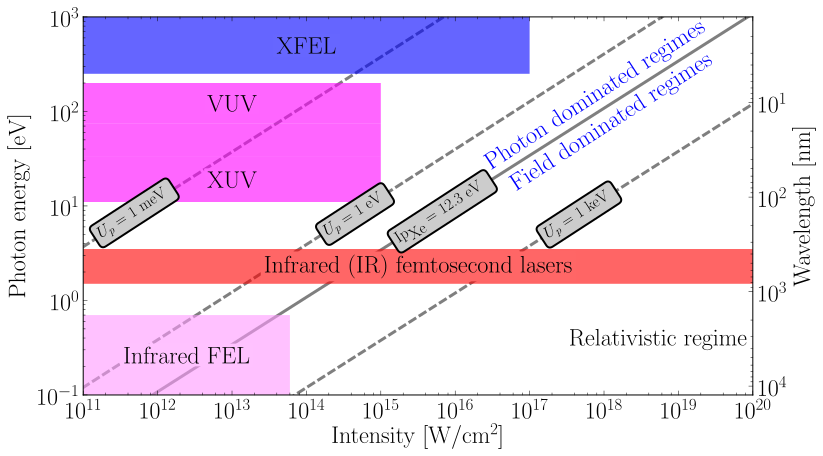
\includegraphics[width=\figurewidth]{figures/regimes}
\caption{Wavelength and intensity regimes. For xenon, lower right half is dominated
         by field processes while upper left half by photon processes. Diagonal
         lines represent constant ponderomotive potential $U_p$. The
         demarcation between the two halves happens when the ponderomotive
         potential equals the ionization potential ($U_p = Ip$).
         Note that the present work concentrate on the VUV and XUV regimes
         where photon processes dominates (at the studied intensities).}
\label{fig:regimes}
\end{figure}

In table \ref{tab:ips} the first ionization energies for the different
rare gas elements used in this thesis (argon and xenon) are shown. As can be
seen from the table and figure \ref{fig:regimes}, xenon and argon can be
single-photon ionized in the VUV regime where photons of 15.76 (for argon)
and 12.13 eV (for xenon) are possible. While xenon's 5p states have the smallest
Ip's, the cross-section for photoionization of the 4d shell is approximately ten
times larger at 13.7 nm (90.5 eV) -- the so called xenon giant 4d
resonance\cite{Becker1986} -- making ionization of these inner-shells
possible\cite{Thomas2009,Ackad2013}.
% http://photon-science.desy.de/news__events/research_highlights/archive/flash_excites_giant_atomic_resonance/index_eng.html

\begin{table}
\begin{center}
\begin{tabular}{ccccccc} \hline
 & \mc{3}{c}{Argon} & \mc{3}{c}{Xenon} \\
Z &
Configuration
        & Ip [eV]
                    &$\lambda$ [nm]
                                & Configuration
                                        & Ip [eV]
                                                    & $\lambda$ [nm] \\ \hline
% Used in the code:
% 16.00   & 77.49             & 12.265625 & 101.1 \\
% 32.34   & 38.34             & 21.390625 & 57.96 \\
% 48.68   & 25.47             & 31.296875 & 39.62 \\
% 65.02   & 19.07             & 41.859375 & 29.62 \\
% 81.56   & 15.20             & 55.015625 & 22.54 \\ \hline
%
% Experimental data (from NIST):
% http://physics.nist.gov/PhysRefData/ASD/levels_form.html
0 & 3p$^5$  & 15.7596109& 78.6721   & 5p$^6$& 12.129843 & 102.214 \\
1 & 3p$^4$  & 27.62967  & 44.8736   & 5p$^5$& 20.975    & 56.4 \\
2 & 3p$^3$  & 40.735    & 30.4368   & 5p$^4$& 31.05     & 39.9305 \\
3 & 3p$^2$  & 59.58     & 20.8097   & 5p$^3$& 42.20     & 29.3801 \\
4 & 3p$^1$  & 74.84     & 16.5666   & 5p$^2$& 54.1      & 22.9176\\
5 & 3s$^2$  & 91.290    & 13.5814   & 5p$^1$& 66.703    & 18.5875 \\
6 & 3s$^1$  & 124.41    & 9.96577   & 5s$^2$& 91.6      & 13.5354 \\
7 &  &  &   & 4d$^{10}$ & 105.978   & 11.699 \\
8 &  &  &   & 4d$^{9}$  & 179.84    & 6.89414 \\
9 &  &  &   & 4d$^{8}$  & 202.0     & 6.13783 \\
10 &  &  &   & 4d$^{7}$  & 229.02    & 5.41368 \\
11 &  &  &   & 4d$^{6}$  & 255.0     & 4.86213 \\
12 &  &  &   & 4d$^{5}$  & 280.9     & 4.41382 \\
13 &  &  &   & 4d$^{4}$  & 314.1     & 3.94728 \\
14 &  &  &   & 4d$^{3}$  & 342.9     & 3.61575 \\
15 &  &  &   & 4d$^{2}$  & 374.1     & 3.3142 \\
16 &  &  &   & 4d$^{1}$  & 403.9     & 3.06968 \\ \hline
\end{tabular}
\caption{First few ionization potentials for (atomic) rare gas elements.
         Source: NIST\cite{NIST}}
\label{tab:ips}
\end{center}
\end{table}

Let us now turn to a more detailed examination of the different mechanisms
present in the different regimes, as well as some regime-independent processes.



\subsubsection{Long wavelength: The IR regime}
\label{section:intro:mechanisms:ir}

Most femtosecond lasers are Ti:sapphire that have a wavelength centred around 800 nm.
This type of lasers sparked the research on clusters. They cover a wide range of
intensity and as such can touch different regimes, from the photon-dominated
one at low intensities to the field-dominated one at larger intensities and
even going up to where relativistic effects cannot be neglected.

One can see how much work was done in the field-dominated (IR) regime over the
years by looking at the wide literature on the subject, see for example ref.
\cite{Fennel2010} or \cite{Ramunno2008}. On the opposite, the VUV and XUV regime
-- the photon-dominated one -- is much less explored and is thus the main
aspect of the present work. Some effects in the IR are still presented here
for clarity. These processes are dominant in the field-dominated regime (see
figure \ref{fig:regimes}).


\subsubsubsection{Above Threshold Ionization (ATI)}

Above Threshold Ionization (ATI) was one of the first observed effects of
intense laser-matter interaction in 1979\cite{Agostini1979}.
In ATI, more photons are absorbed by atoms
than is normally required to ionize it. This results in photoelectrons spectra
showing peaks at energies much larger than expected separated by the photon
energy. Because it's a multiphoton process, ATI requires large
intensities~($\gamma \ll 1$)\cite{Krainov1997,Lewenstein2008}.


\subsubsubsection{Tunnel ionization}

The most striking effect in the IR regime is tunnel ionization\cite{Niikura2009}.
The Coulomb potential of an atom can be bent enough by the (oscillating) laser
field and the probability of a bound electron tunnelling out becomes significant,
as shown on figure \ref{fig:ionization:tunnel}. Tunnel ionization is also
sometimes called optical field ionization (OFI), or more simply field
ionization, since one can describe the process as the laser field as the source
of the potential bending and ionization.
\lrnote{I made the change to the last sentence, but
am still not happy with it. it's b/c the laser field picture is really only a
semiclassical quantum picture in the length gauge. i will clarify more when we
talk and maybe we can edit it appropriately then.}


% Above Threshold Ionization (ATI) https://en.wikipedia.org/wiki/Above_Threshold_Ionization_%28ATI%29
% Strong Field Approximation (SFI)
% http://massey.dur.ac.uk/resources/cpchirila/
\begin{figure}
 \centering
 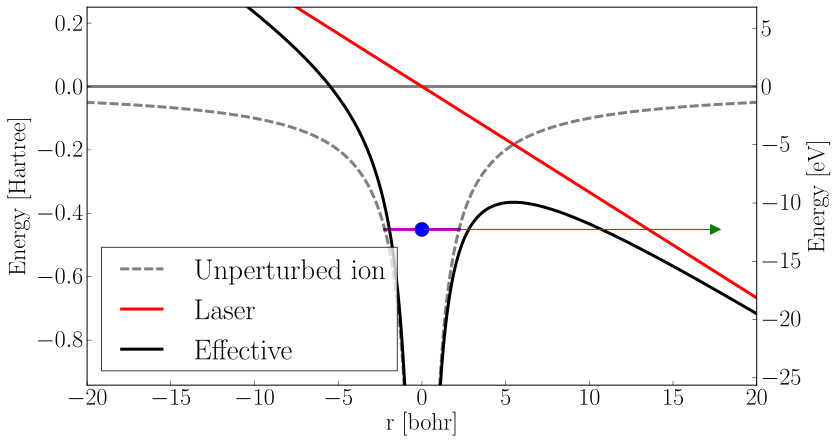
\includegraphics[width=\figurewidth]{figures/ionization_tunnel}
 \caption{\label{fig:ionization:tunnel}Tunnel ionization. The potential
          due to the laser (red) bends the unperturbed ion potential
          (grey dashed). The electron (blue dot) sitting at the unperturbed
          eigenvalue (magenta) now has a probability to tunnel through the total
          potential barrier (black line). The laser frequency must be small
          enough for the probability to be non-negligible (large wavelength)
          and intensity large enough ($\gamma \ll 1$).}
\end{figure}

Tunnel ionization is at the heart of High Harmonic Generation (HHG) and
attosecond science\cite{Fennel2010}. A laser pulse, normally in the IR regime,
bends the atomic potential bounds electrons are feeling, allowing them to tunnel
out. They are then accelerated in the laser field where they gain energy.
As the laser field changes direction within a laser cycle, electrons are forced
back onto their parent ion where they can
recombine and emit high energy photons. The emission spectra,
containing only odd harmonics, shows an intensity decrease as a function of
harmonic number, followed by a plateau and a cutoff. Since the description
of the phenomena in 1993\cite{Corkum1993}, HHG studies expended into its own
sub-field. For example, Murphy \textit{et al.} used the 21st harmonic of a
800 nm Ti:sapphire to ionize xenon clusters\cite{Murphy2008a,Murphy2008b}
with these new 32.6 eV (38 nm) photons.
For more details on HHG see references~\cite{Levesque2006} and
\cite{Lewenstein2008}.
\lrnote[noinline,margin]{you should be prepared to answer "why only odd harmonics?"}


\subsubsubsection{Inverse Bremsstrahlung Heating}

Once electrons are created in the IR regime they can continue to absorb energy
from the laser.
Inverse Bremsstrahlung Heating (IBH) is the inverse process of Bremsstrahlung
where an electron emits a photon when deflected, either by a heavier ion in the
case of plasma, or by magnetic fields in the case of synchrotrons. IBH is thus
the absorption of photons accelerating the electrons\cite{Schlessinger1979}.

For large frequencies, the quiver amplitude of equation \eqref{eqn:quiver} is
small; the electric field oscillates
too rapidly for the electrons to gain significant acceleration. On the other
hand, for smaller frequencies (larger wavelengths) the quiver amplitude can
be significant. In the case of IR, electrons can be pushed outside the cluster
and back in; at $\ten{3}{16}$~W/cm$^2$ and 800~nm, the quiver
amplitude is $x_q \approx 500 a_0$, where $a_0$ is the Bohr
radius\cite{Georgescu2007}, while a Xe$_{1,415}$ cluster is~115~$a_0$.

The linear momentum gained by electrons in the laser field is then redistributed
as thermal energy by collisions and scattering on heavier ions.
IBH plays an important role in the IR regime where the laser field easily
drives the electrons through the cluster\cite{Fennel2010}.

% The energy $E$ change rate over time due to IBH is given\cite{Fennel2010} by:
% The IBH rate is given\cite{Fennel2010} by:
The rate of change of energy $E$ over time due to IBH (per electron) is
given\cite{Fennel2010} by:
\begin{align}
\left< \dt{E} \right> & = 2 U_p \frac{\tau \omega^2}{\tau^2 \omega^2 + 1},
\end{align}
where $\tau$ is the inverse of the electron-ion collision frequency, $\omega$ the
angular frequency of the laser and $U_p$ the ponderomotive potential.

\fxnote{According to Bostedt2010\cite[page 3]{Bostedt2010}, IBH scales as
$\lambda^{8/3}$ and cites Krainov2000\cite{Krainov2000} and
Krainov2002\cite{Krainov2002}}
% ? can you explain the problem to me when we talk next?

\subsubsection{Shorter wavelengths: Into the VUV and XUV regime}
\label{section:intro:mechanisms:vuv}

% http://www.laserfocusworld.com/blogs/what-the-hecht/2012/05/euv-xuv-acronym.html
% http://www.spacewx.com/Docs/ISO_PRF_21348_e_review.pdf
% http://www.iso.org/iso/home/store/catalogue_tc/catalogue_detail.htm?csnumber=39911

With the help of new FEL facilities, high laser intensities can be reached at
lower wavelength (and thus larger photon energy) than with traditional
femtosecond lasers. \textit{Vacuum ultraviolet} (VUV) radiation, ranging from 200 to
10~nm (6.2 to 124~eV), is normally absorbed by the atmosphere. Studying them
requires vacuum chambers (hence the name) or a pure nitrogen propagation medium.
At short wavelengths, the photons can start to ionize inner shell electrons. In
that case, the term \textit{extreme ultraviolet} (XUV, or EUV) is used. XUV wavelengths
range from 121~nm (hydrogen's Lyman alpha line, 10.25 eV) to 10~nm (124~eV).
As the two regimes have overlapping wavelengths, they are often used
interchangeably but XUV is generally used with wavelengths where no
material is known to be transparent\cite{Laane2009}. Note that in other fields
XUV can be used to describe soft X-rays\cite{Eichmeier2008,iso21348}

At relatively low intensity (less than 10$^{14}$~W/cm$^2$
\cite{Ramunno2008}), in the photon-dominated regime, atoms and ions
can be ionized by photon absorption. If the photon energy is more than the
electron's biding energy (see table \ref{tab:ips} for numerical values) single
photon ionization will be the dominant energy transfer mechanism.

While not as strong as in the IR regime, IBH is still important in the
VUV\cite{Krainov2000} up to 62 nm\cite{Georgescu2007}.


\subsubsubsection{Photon absorption}

Initially described by Einstein as the photoelectric effect, a bound electron
absorbs a photon from the laser and is promoted to the continuum where it is
free to leave its parent ion. Figure~\ref{fig:ionization:single} shows a
schematic of the mechanism. For example, the first energy level of atomic
xenon is at -12.27 eV requiring a photon wavelength equal or shorter than
101.1 nm for ionization.


\begin{figure}
 \centering
 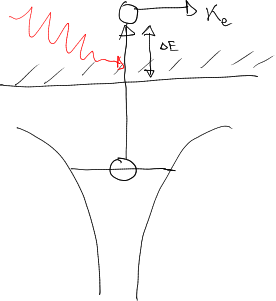
\includegraphics[width=\figurewidth]{figures/ionization_single}
 \caption{Single photon ionization for the atomic, isolated model. A photon
          (red) is absorbed by a bound electron (blue) which gets promoted to
          the continuum. The remaining energy $\Delta E$ between the photon's
          and the Ip results in electron's kinetic energy $K_e$.
          Chapter \ref{section:tools} describes the cluster environment
          influence.}
 \label{fig:ionization:single}
\end{figure}

If the photon energy exceed the electron's binding energy, the difference in energy
will be transferred as extra kinetic energy in the
resulting photoelectron. This can thus be used to sample the states in the
target by measuring the photoelectron energy spectrum\cite{Fennel2010}.

However, if the photon energy is less than the binding energy, then a single
photon cannot ionize an atom. If the intensity is large enough though, the
photon density will be sufficient that many photons can be absorbed during a
small time interval.
This effect is called multiple-photon ionization (MPI, not to
be confused with the Message Passing Interface used in parallel programming) and
is a non-linear process. The ionization rate of $\nu$-photons MPI is given
by\cite{Fennel2010}:
\begin{align}
\Gamma_{\nu} = \sigma_{\nu} I^{\nu}.
\label{eqn:ionization:rate:mpi}
\end{align}
Being a nonlinear process, multi photon ionization is present at larger
intensities than single photon ionization. But being photon processes, both are
superseded by tunnel ionization at even larger intensities (or when
$\gamma~\gg~1$).


% \clearpage
\subsubsubsection{Auger effect}

At even shorter wavelength, the photon energy might be large enough not only
to ionize the highest energy electron but also some inner-shell electrons.
When such an inner shell electron gets ionized, it leaves a hole; the atom is
thus in an excited state. An outer shell electron will then transition by
\textit{Auger decay} to the hole. The transition energy is used by a third
electron (the Auger electron) to leave the ion, leaving the latter
doubly-ionized. Figure \ref{fig:auger} shows a diagram of the process.

\begin{figure}
 \centering
    \begin{subfigure}{0.48\columnwidth}
        \centering
        \includegraphics[width=\textwidth]{figures/auger_step_1}
        \caption{Step 1: An xenon 4d inner shell electron absorbs a high
                 energetic photon and leaves the atom. \\}
        \label{fig:auger:1}
    \end{subfigure}
    \begin{subfigure}{0.48\columnwidth}
        \centering
        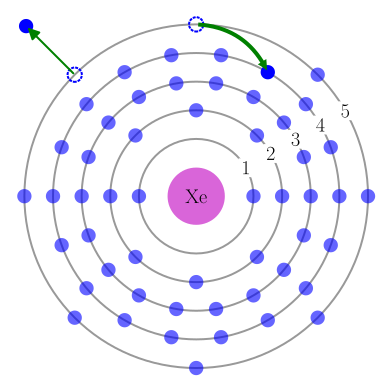
\includegraphics[width=\textwidth]{figures/auger_step_2}
        \caption{Step 2: An outer shell electron decays into the created hole,
                 transferring the energy difference between the two states to a
                 third electron which is ejected (the Auger electron).}
        \label{fig:auger:2}
    \end{subfigure}
        \caption{\label{fig:auger}Auger ionization of a xenon 4d electron by a
                 high energetic X-ray photon. Xenon's 54 electrons are shown
                 as blue dots with the distance to the core representing their
                 principal quantum numbers $n$.}
\end{figure}

To access core electrons, photons must be highly energetic, normally in X-rays.
While not the focus of the present work, an interesting aspect is that xenon
atoms have a giant resonance of the (inner-shell) 4d state; the cross-section of
photoionization of the 4d electron is ten times larger than the
one of valence  electrons at 13.7 nm wavelength~(90.5~eV)\cite{Becker1986}.
This process was included in the model for a comparison with a 2009 experiment
by Thomas \textit{et al.}\cite{Thomas2009} on xenon clusters at FLASH-DESY.
The German group saw clusters becoming nanoplasmas from which the outer shells
ions undergo Coulomb explosion while the relatively neutral core expands
hydrodynamically. These results could be reproduced by our model in a recently
published article entitled ``Recombination effects in soft-x-ray cluster
interactions at the xenon giant resonance'', published in May 2013 in
\textit{New Journal of Physics}\cite{Ackad2013} and included in chapter
\ref{section:papers:recomb}.

% ******************************************************************************
\subsubsection{Regime independent processes}
\label{section:intro:mechanisms:noregime}

Once electrons are created in the cluster, other mechanisms appear. During
impact ionization a first electron collides with an atom and, if it has enough
kinetic energy, will transfer a portion of it to a bound electron, promoting it
to the continuum. Figure \ref{fig:ionization:impact} shows the energy diagram
of the process.

\begin{figure}
 \centering
 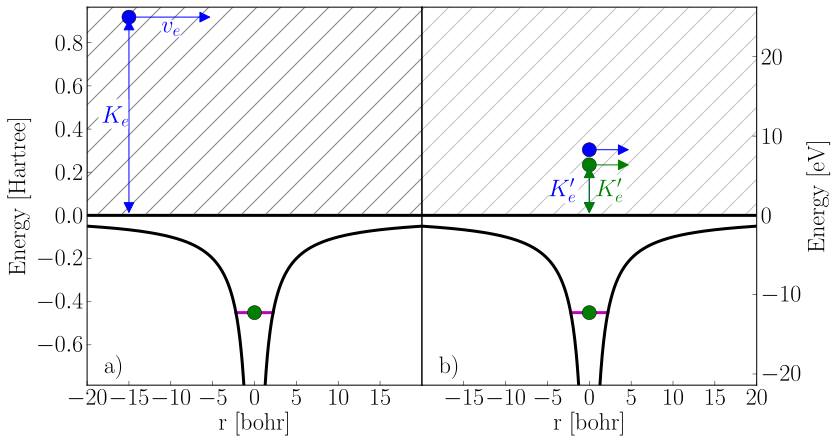
\includegraphics[width=\figurewidth]{figures/ionization_impact}
 \caption{Impact ionization. The colliding electron (blue dot) gives a portion
          of its energy to a bound electron (green dot), promoting it to the
          continuum.}
 \label{fig:ionization:impact}
\end{figure}

Impact ionization can be modelled through cross-sections. These
cross-sections are normally obtained from the semi-empirical Lotz
formula\cite{Lotz1967}:
\begin{align}
\sigma & = \sum_{i}^{N} a_i q_i \frac{\ln{\pa{E/\textrm{Ip}_i}}}{E \textrm{Ip}_i} \pa{1 - b_i
\ex{-c_i \pa{E/\textrm{Ip}_i - 1}}},
\label{eqn:impact:ionization:lotz}
\end{align}
where Ip$_i$ is the ionization potential of the $i^{\textrm{th}}$ shell and $E$
the impacting electron's kinetic energy \textit{at infinity} (or above threshold).

\subsubsection{New regime, new processes}
\label{section:intro:mechanisms:new},

By going to shorter wavelengths, FEL installations allowed experiments at high
intensities in the VUV and XUV regime. These experiments saw surprisingly
high charge states as the results of the clusters
explosion\cite{Wabnitz2002,Bostedt2010}. For example, Wabnitz \textit{et al.}
saw, at FEL-DESY, Xe$^{4+}$ when Xe$_{80}$ clusters were irradiated with 98 nm,
100 fs FEL pulses of, what was though at the time, $\ten{2}{13}$~W/cm$^2$
intensity. For larger clusters (Xe$_{30,000}$), xenon ions up to
Xe$^{8+}$ were observed. This was a big surprise considering that the 98~nm
photons (12.7 eV) could only ionize neutral xenon to Xe$^{1+}$ by itself;
data showed that up to 30 photons were absorbed per atom for the largest
clusters. Using a different source of photons and at a different wavelength
(21st harmonic of an 800 nm Ti:sapphire, XUV: 32.6 eV, 38 nm),
Murphy \textit{et al.} observed the same pattern of high charge states in xenon
clusters\cite{Murphy2008a,Murphy2008b}.

Such high charge states could not be explained by the previous processes only.
New mechanisms were thus proposed to explain these surprising results.
The four main models proposed throughout the years are covered next.


\subsubsubsection{Atomic potentials}

First, Santra \& Greene proposed using \textit{atomic potentials} instead of
the Coulomb potential in a rate equation model (with infinite spatial
extension and
constant density) as seen on figure \ref{fig:heating:atomic_pot}.
The atomic nucleus is normally shielded by bound electrons but inside the
electronic cloud the shielding disappears and the nucleus potential is more
important. If an impacting electron can get close enough to the core, it will
feel the unshielded potential.
In reference \cite{Greene2003}, Santra \& Greene used an approximated form for
the atomic potential, fitting one parameter with the first ionization potential.
A later\cite{Walters2006} publication used a
potential shape generated by the code written by Herman and
Skillman\cite{HS1963} (HS) to describe a more realistic
potential, based on a
Hartree-Fock formulation. Using these atomic potentials, they saw Xe$^{3+}$,
Xe$^{5+}$ and Xe$^{7+}$ for intensities of $\ten{1.4}{12}$, $\ten{1.4}{13}$ and
$\ten{7.3}{13}$~W/cm$^2$ respectively for Xe$_{1,500}$ clusters, similarly to
what was seen in at FEL-DESY.

\newpage
\subsubsubsection{Barrier suppression}

Another model proposed by Siedschlag and Rost\cite{Siedschlag2004} in 2004 was
the barrier suppression in single photon absorption which is shown on figure
\ref{fig:heating:barrier}. Due to the proximity
of neighbours, the potential barrier between them is lowered and
a photo-transition to the continuum becomes possible, even with a single photon.

\lrnote{nic, did we ever talk about the downsides of the rost model?}

\subsubsubsection{Many-Body Recombination}

\textit{Many-Body Recombination} (MBR) was proposed in 2005\cite{Jungreuthmayer2005}
as a simple mechanism to explain the high charge states seen in the
experiments at FEL-DESY. In a strongly coupled plasma, electrons can recombine
easily to a high excited
state after collisions with many bodies. Later, these newly bound electrons can
absorb a new photon from the laser field for another transition to the
continuum -- see figure \ref{fig:heating:mbr}.
Because MBR is much more efficient than three-body
recombination (due to the large density of charged particles), much more
photons are absorbed this way. It was also shown that MBR deposited more energy
in the clusters than traditional IBH.
The simplicity of the
method lies in the fact that in a classical MD simulation, MBR is automatically
included without extra implementation as the high excited states have energies
which are close to each other and can thus be treated classically.
Jungreuthmayer \textit{et al.} were able
to see Xe$^{3+}$, Xe$^{5+}$ and Xe$^{7+}$ for intensities of $\ten{1.5}{12}$,
$\ten{1.5}{13}$ and $\ten{7}{13}$~W/cm$^2$ respectively when simulating
Xe$_{1,000}$ clusters.

\begin{figure}
 \centering
    \begin{subfigure}{0.48\columnwidth}
        \centering
        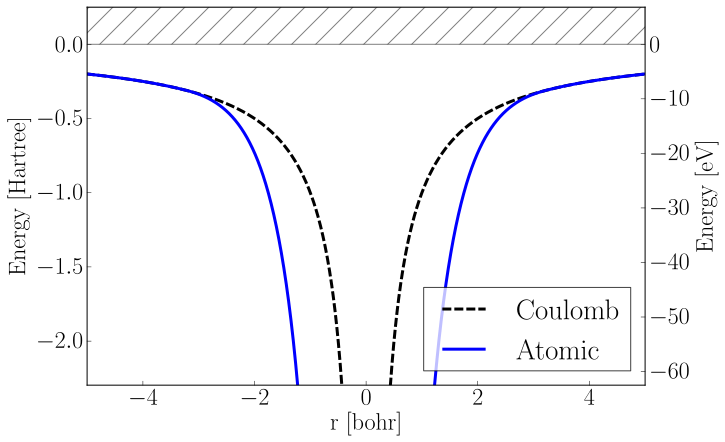
\includegraphics[width=\textwidth]{figures/heating_atomic_potential}
        \caption{Atomic potential (blue line) drops faster than Coulomb one
                (black dashed line), allowing more energy absorption through
                IBH.\\}
        \label{fig:heating:atomic_pot}
    \end{subfigure}
%
    \begin{subfigure}{0.48\columnwidth}
        \centering
        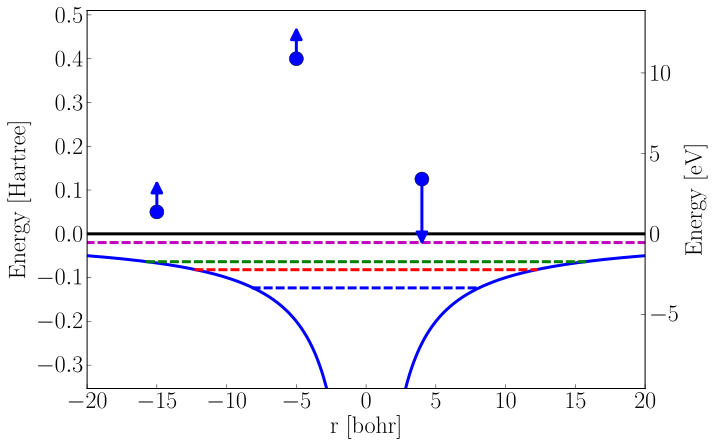
\includegraphics[width=\textwidth]{figures/heating_mbr}
        \caption{MBR: energy exchange between free electrons during collisions
                 makes one recombine to a highly excited state where it can
                 reabsorb a new photon from the laser field.}
        \label{fig:heating:mbr}
    \end{subfigure}
\\
    \begin{subfigure}{\figurewidth}
        \centering
        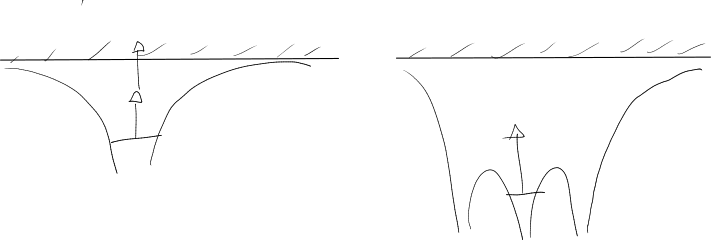
\includegraphics[width=\textwidth]{figures/heating_barrier_sup}
        \caption{Barrier suppression between ions in a cluster environment allows
                 a single photon to ionize deeper levels (right), not accessible
                 with a single atom (left).}
        \label{fig:heating:barrier}
    \end{subfigure}
 \caption{More heating mechanisms}
 \label{fig:heating}
\end{figure}


\clearpage
\subsection{Contributions of thesis}

The goal of the current thesis is to acquire a better understanding of
laser-matter interaction.
More specifically, the
question of \textit{how} the energy is deposited in a nanoscale object
--a rare gas cluster-- by an
ultra-short and ultra-intense laser pulse will be studied. This interaction
largely depends on the specific target material and on the pulse's wavelength
and duration, both defining the interaction regime. A specific regime will
thus be targeted; mainly short wavelengths, from VUV to XUV, as many questions
raising from recent experiments are still debated.

While many tools exist to study laser-mater interaction, only classical
approaches can be considered as a full quantum calculation, even
with some degree of approximations, is not possible. Clusters become
nanoplasmas quite rapidly and have large charge and field fluctuations inside
them. This and their finite nature makes it hard to use tools such as rate
equations to model them. Pure classical simulations allows for relatively large
systems to be simulated and are thus the tool of choice.

\lrnote{also remind me to talk to you about justifications of classical
regmies in plasma physics... we might add that discussion here.}

\subsubsection{Tools}

First, chapter \ref{section:tools} describes the different tools and models
that were developed and implemented to answer our questions. While chapter
\ref{section:tools:md} concentrate on the classical aspect of the problem,
chapter \ref{section:tools:qfdtd} describes in detail a quantum approach that
was used named QFDTD for Quantum Finite-Difference Time-Domain.
Note that all implementations used are original work; all code packages
were developed from scratch by me or under my direction and no external packages
were used. The MD package described in
chapter \ref{section:tools:md} ($\sim$16k lines of code) contains 86~\% of code
written by me, 12~\% by Edward Ackad (postdoctoral fellow) and smaller contributions from
Julien Roy (undergraduate student) during his summer 2012 internship. Furthermore, the QFDTD package
($\sim$16k lines of code) contains 3~\% of code written by Stan Hatko (undergraduate student) while the
rest is my original work. Most tools were written in C++ with Python being used
for analysis and plotting.

For libraries described in chapter \ref{section:tools:libraries}, 79~\% of the
ionization library was written by me, 20~\% by Edward Ackad and smaller
contributions from Stan Hatko during his summer 2012 internship. All other
libraries described in chapter \ref{section:tools:libraries} were fully
written and developed by me.

All these powerful tools were extremely useful for my studies and will also allow
the group to continue its investigation of laser-clusters interaction even
after my departure.

Additionally to the models described in
chapter \ref{section:intro:mechanisms}, a notable new one was
developed that revealed be of great importance in the description of
laser-clusters interaction. This new model is discussed next.


\subsubsection{Augmented Collisional Ionization (ACI)}

Wabnitz's \textit{et al.} experiments at FLASH-DESY in 2002 revealed the
interestingly high charge states in xenon clusters. Since then, different groups
proposed models to explain these results as described in chapter
\ref{section:intro:mechanisms:new}.
Then, in 2010, Bosted \textit{et al.}
re-calibrated the intensity used during the 2002 experiments.
Instead of the previously thought $\ten{2}{13}$~W/cm$^2$, the intensity was
re-calibrated to $\ten{8}{12}$~W/cm$^2$, less than half of the initial value.
Additionally, the largest clusters was tripled in size, from Xe$_{30,000}$
to Xe$_{90,000}$.
Could the different models still produce the same amount of high charge states
at the new, lower intensities?

Additionally, in 2008 experiments \cite{Bostedt2008,Murphy2008b} were performed
in the XUV regime near 30~nm~(41~eV). At this wavelength, the photon energy is
too small for inner shell ionization of rare gas atoms, yet too large
(at reported intensities) for any appreciable laser-field-driven processes, such
as collisional heating, that dominate intense laser-cluster interactions at
longer wavelengths. This presents the opportunity to isolate the influence of
the internal electronic structure from the laser-cluster interaction.

Our group thus proposed a new mechanism for energy transfer from the laser field
to the cluster via two-step collisional ionization. With this two-step model, an
electron might not have enough kinetic energy to directly collisionally ionize
an atom (or ion), but it could still transfer some of
its energy to promote a bound electron to an excited state. Once an atom is
excited, it becomes easier to ionize, due to the large cross-sections of excited
atoms and ions, by subsequent impact from a low energy electron. This gives the
opportunity for low energy electrons to still participate in the cluster
ionization, giving the name \textit{augmented collisional ionization} (ACI) to
the process.

\begin{figure}
 \centering
 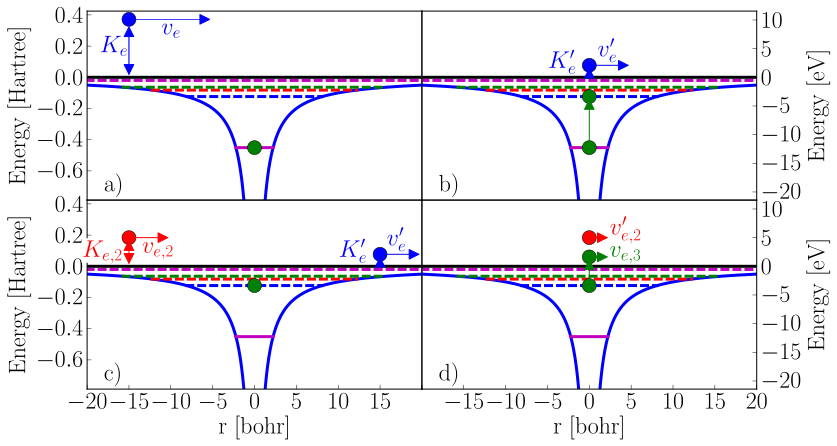
\includegraphics[width=\figurewidth]{figures/ionization_aci}
 \caption{ACI. First electron (in blue) collides with ion in a) and gives
          $K_1$ energy for the transition of a bound electron (in green) to an
          excited state in b).
          A third electron (in red) collides with the ion in c) and
          gives the remaining $K_2$ necessary for the transition to continuum
          in d). The first step is a) to b) and the second step is from c) to d).}
 \label{fig:ionization:aci}
\end{figure}

% \begin{figure}
%  \centering
%     \begin{subfigure}{0.48\columnwidth}
%         \centering
%         \includegraphics[width=\textwidth]{figures/aci_0}
%         \caption{Before}
%         \label{fig:ionization:aci:0}
%     \end{subfigure}
%     \begin{subfigure}{0.48\columnwidth}
%         \centering
%         \includegraphics[width=\textwidth]{figures/aci_1}
%         \caption{1. }
%         \label{fig:ionization:aci:1}
%     \end{subfigure}
% \\
%     \begin{subfigure}{0.48\columnwidth}
%         \centering
%         \includegraphics[width=\textwidth]{figures/aci_2}
%         \caption{2. }
%         \label{fig:ionization:aci:2}
%     \end{subfigure}
%     \begin{subfigure}{0.48\columnwidth}
%         \centering
%         \includegraphics[width=\textwidth]{figures/aci_3}
%         \caption{3. }
%         \label{fig:ionization:aci:3}
%     \end{subfigure}
% \caption{ACI. First electron (in blue) gives $K_1$ energy for the transition
%           to an excited state. Second electron (in green) gives the remaining
%           $K_2$ necessary for the transition to continuum.}
% \label{fig:ionization:aci}
% \end{figure}


Figure \ref{fig:ionization:aci} shows an energy diagram of ACI and the
different transitions possible. This two-step model is implemented using
cross-sections for collisional transition (ground state to excited state and
excited state to continuum), similarly to traditional impact
ionization. See chapter \ref{section:intro:md:cross-sections} for more
details on cross-sections.

The ACI model revealed to be an important contribution to the field. As will be
seen from the publications, experimental results can be reproduced with this
model.



\subsubsection{Publications}

After the tools are presented in chapter \ref{section:tools}, the present thesis
consists of a series of four published articles and one article in preparation
where the models and tools are tested and used.


\subsubsubsection{ACI introduction paper}

First, the work on excited states and ACI in clusters was published in the article
``Augmented collisional ionization via excited states in XUV cluster
interactions'' published in 2011 in \textit{Journal of Physics B: Atomic,
Molecular and Optical Physics}\cite{Ackad2011a} and can be found in chapter
\ref{section:papers:aci} (page \pageref{section:papers:aci}). Argon clusters
(Ar$_{80}$ and Ar$_{147}$) were simulated with parameters used in experiments
at FLASH-DESY in 2008 by Bosted \textit{et al.}\cite{Bostedt2008}.
(32.8 nm -- 37.8 eV, 25 fs and intensities from $\ten{5}{13}$ to
$10^{14}$~W/cm$^{-2}$). It was found that not only ACI could explain the
Ar$^{4+}$ seen at FLASH but also that it
was a dominant process, happening more often than traditional impact ionization.
Due to the efficiency of ACI, high charge states can be reached in shorter time
than previously though which can have a significant impact on biomolecules
imaging. This first ACI article was a stepping stone in the current work as it
showed the validity of the model, as simple as it could be.


\subsubsubsection{Cluster size influence}

Next, chapter \ref{section:papers:size} presents the article ``Clusters in
intense XUV pulses: Effects of cluster size on expansion dynamics and
ionization''. Also published in 2011 (\textit{Physical Review~A}\cite{Ackad2011b}),
argon clusters were simulated in the XUV regime (32.8 nm,
I~=~$\ten{5}{13}$~W/cm$^{2}$, 25 fs) with cluster sizes from Ar$_{55}$ to
Ar$_{2,057}$. It was found that the dynamics is highly collisional and
larger clusters even more so. By rapidly ionizing the lower charge states,
collisional processes will prevent photo-ionization even before the laser pulse
is finished. This mechanism was called \textit{collisionally reduced photoabsorption}.
The amount of energy absorbed through photo-ionization by Ar$_{55}$ clusters was
reduced by 30~\% and 45~\% by Ar$_{2,057}$ clusters when collisional processes
are included.
Higher charge states are more abundant and also appears sooner during the
dynamics in large clusters compared to smaller ones. ACI is vital for the
description; 20~\% of ions are in an excited state after the laser peak.
During the laser pulse, the distribution of charge inside clusters is
relatively isotropic but as the simulation evolves, the outer shells tend to
lose electrons more than the core and eventually disintegrate through Coulomb
explosion.
The core stays relatively neutral and expend thermodynamically.

The ion kinetic energy distribution revealed that Ar$^{2+}$  provided most of
the high energy tail. Additionally, the highest charge states had the least
energy. The highest charges states being created in the (neutral) core, the
electrons shield these high charge states, preventing them from accelerating
as much as the outer shells ions.

Electrons thermalize rapidly to a Maxwellian distribution. The larger clusters'
distribution are isotropic due to the high collisional rates while smaller
clusters keep the anisotropy coming from photoionization.



\subsubsubsection{Revisiting the 100 nm experiment}

Afterwards, chapter \ref{section:papers:100nm} contains the draft of the article
``Augmented Collisional Ionization in the VUV regime; a theoretical study''.
After Wabnitz \textit{et al.}'s
2002 DESY-FEL experiment's intensity was re-calibrated in 2010, we hypothesized
that our ACI model could still explain the high charge states seen in xenon
clusters, even with the lower intensities.
Since the VUV (98 nm, 12.65 eV)
photons cannot ionize a Xe$^{1+}$ to Xe$^{2+}$ (see table \ref{tab:ips} for xenon
ionization potentials), all charge states higher than Xe$^{1+}$ must be created
with other processes.
We included single photon ionization,
impact ionization, ACI and recombination in simulations of Xe$_{80}$ to Xe$_{5,083}$
interacting with DESY's 100~fs laser pulse at different intensities.
We compared our model
with previous work with ACI disabled and found good agreement.
The high performance of my
code implementation (see chapter \ref{section:tools:opencl} on GP-GPU) allowed
running thousands of MD simulations. The chaotic nature of the many-body
problem requires acquiring vast amount of data for valid statistics, giving more
weight to our results. On average, it was found that two more charge states are
accessible when ACI is enabled, a clear indication that ACI has a central role
amongst the ionization channels.

Due to the spacial intensity profile of the laser pulse, simulations were run
at different intensities to simulate the effect of experimental data acquired
from clusters dispersed in the laser's spacial profile. This improves the validity of
simulation data when comparing with experiments.
Our data was in good agreement with the 2002 experiment. Both the dominant
charge states and the highest charge states matched the experiment data. This
was not the case of other models which used the old intensity.

The last part of the article discuss the influence of the potential depth
of equation~\eqref{eqn:md:sigma}.
% Santra and Greene suggested\cite{Greene2003}
% using atomic potentials instead of a pure Coulombic one to explain the high
% charge states seen in experiments.
By allowing deeper potentials in our
simulations, it was hypothesized that larger charge states could be obtained.
The influence of the potential depth used in simulations is often neglected in
the literature. That article section sheds some light on the topic.
Since electrons are now allowed to go deeper in the ions potential well,
recombination must be used to prevent them from having a total energy less than
the ion's eigenvalues which would not be allowed quantum mechanically.



\subsubsubsection{Recombination }

Finally, chapter \ref{section:papers:recomb} present the article ``Recombination
effects in soft-x-ray cluster interactions at the xenon giant resonance''
published in May 2013 in New Journal of Physics.

Xenon atoms have, centred at around 13 nm (95.4 eV), a photoabsorption
cross-section approximately ten times larger for the 4d electrons than for the
outer-most shell 5p electrons; inner shell ionization is thus possible and
Auger processes creates highly charged ions, even in the case of xenon
gas\cite{Uiberacker2007}.

In experiments at 13.7 nm (90.5 eV) by Thomas \textit{et al.} in
2009\cite{Thomas2009}, the amount of Xe$^{1+}$ observed in clusters was
significantly more than in xenon gas, indicating that recombination effects were
important. At the time it was clear that photoabsorption and recombination alone
could not explain by itself these results.

Thomas \textit{et al.}'s experiment was described using our models. Xenon
clusters of sizes 147, 1,415 and 5,083 were simulated under a 13.7 nm
(90.5 eV) laser at different intensities from $\ten{1}{11}$ to
$\ten{5.8}{14}$ W/cm$^2$. Time-of-flight spectra were in good agreement with the
experiment. We also saw that the higher charge states came from the clusters'
outer-shells while the lower charged ions came from the clusters' core. Even
though ions in the neutral core can reach high charge states, they recombine
quickly to lower charge states. The expansion of ionized clusters is best
described by a Coulomb explosion of the outer-shells and a hydrodynamically
expending neutral core.



\subsubsubsection{A quantum approach}

Going further, interesting questions came up. For example, how is a bound
electron's wavefunction affected by a neighbouring ion or the cluster potential?
Due to my background in electromagnetic simulations, I was surprised to read
an article using the FDTD method -- normally used in electrodynamic simulations --
for quantum calculations. I was curious how far could the FDTD method be
applied to quantum problems and if it could answer some of our questions.
A QFDTD simulation package was thus developed, again from scratch,  implementing
two kinds of time evolution; real and imaginary. The model and its implementation details
are discussed in chapter \ref{section:tools:qfdtd}.

The work developed in chapter \ref{section:tools:qfdtd} was published in the article
``Nonlinear grid mapping applied to an FDTD-based, multi-center 3D
Schr\"odinger equation solver'' presented in chapter \ref{section:papers:qfdtd}.
Published in 2012 in \textit{Computer Physics Communications}\cite{Bigaouette2011}, it
explains the QFDTD method and its implementation, with emphasis on the new
nonlinear mapping introduced for faster calculation. The QFDTD package is the
first to use both the real and imaginary time evolution, opening the door to
easily get eigenvalues, eigenstates and their time evolution in a time-dependent
and arbitrary spacial shape potential.
The method was first validated by comparing with the analytic solutions of
the hydrogen atom and then applied to solve the H$_{2}^{+}$ molecule.
Comparison with experimental data was in good agreement for the eigenvalues
while the eigenstates could be visualize easily. A new method to calculate
eigenstates is also presented in the article. The publication also
describes in detail the nonlinear mapping that allows reducing both the memory
usage required to store the grid and the time required to calculate the time
evolution. The method is a generic way to obtain a nonuniform grid with cells
concentrated around multi-centres of interest for used in any (finite difference
based) partial differential equation solvers.

Before listing the different publication of the current thesis, the different
methodology and tools used and developed throughout the years will be presented
and discussed.




\clearpage
\section{Methodology and Tools}
\label{section:tools}

A large selection of methods exist to study laser-cluster interaction,
differentiating themselves through the amount of approximation taken.

Exact solution of the quantum mechanical system is, most of the time,
intractable. Theoretical investigations thus require some degree of
approximation, a compromise between feasibility and exactitude. On one end of
the spectrum, the most general methods are solving the
Time-Dependent \schrodinger Equation (TDSE) directly and Quantum Monte-Carlo
(QMC) methods\cite{Nightingale1998}. Unfortunately, these methods can only be applied to the simplest
systems of small numbers of electrons; clusters cannot be studied using these
methods.

Larger systems can be studied using \textit{ab initio} methods (``from
first principles'') which covers a wide range of techniques. In this class of
methods one can find \textit{Hartree-Fock} (HF) methods which consist on
approximating the ground state wavefunction by a single Slater
determinant\cite{Laaksonen1986,Schafer2009}.
In HF methods, instantaneous electron-electron Coulomb repulsion is not
included directly in the system's Hamiltonian. Instead, only the average field
resulting from other electrons is used, giving the often used name of
\textit{self-consistent field} methods. Other \textit{ab
initio} methods are the \textit{Post Hartree-Fock} methods where electron
correlation is added\cite{Cramer2004}. An example is the \textit{Configuration Interaction} (CI)
method. Because of their great accuracy, these methods are restricted to
relatively small systems, generally less than 10 atoms. Full \textit{ab initio}
treatment of clusters is also not possible.

Larger systems require
more approximations. \textit{Density Functional Theory} (DFT)
is an often used method for cluster studies requiring quantum aspects, with
either quantum or semiclassical propagation\cite{Schafer2009,Fennel2010}.
It starts by formulating an
expression for the total energy of electrons and ions and derives static and
dynamic equations from it. All approximations are done in the selection of this
(energy) functional. The upper limit on these methods is of practical reasons,
mainly computational power available. On the other side, because the chosen
functional approximate the underlying quantum system, specific quantum effects
might not be included, for example shell effects or tunnelling are neglected.

Because DFT methods are mean field in nature, they cannot account for the large
field fluctuations seen in strong field cluster dynamics.

Continuing on the spectrum of methods, classical methods likes Molecular
Dynamics (MD) solves Newton
equations of motion with any kind of forces between particles\cite{Skeel1998}.
When used in
laser-cluster simulations, MD generally uses the instantaneous electrostatic
(Coulomb) force between charged particles. MD codes have the advantage of being
straightforward to implement and use, give macroscopic properties easily and allow a
relatively large amount of particles to be simulated, while still allowing
specific quantum treatment when necessary (for ionization events for example). For
these reasons it is the method of choice for use in the present work.

A limitation of MD is that it cannot account for field propagation effects. For
large clusters of more than tens of thousands of atoms, these effects can become
important. Particle-in-cell (PIC) methods, where particles interact with a grid which propagates the
electromagnetic field (through Maxwell's equations) that other particles see
intrinsically describe these retardation effects. PIC can be successfully used
to model large clusters, but they tend to be more complex and so lack the
simplicity of MD. Additionally, because they treat particles to be of the same
size as the underlying grid, they do not describe close range interactions.
Nevertheless, Varin \textit{et al.} developed a new method that add microscopic
corrections to PIC close range interactions\cite{Varin2012}. With these microscopic
corrections, collisions between particles are described similarly to MD, insuring
a better description of the dynamics. This MPIC method has great prospects
as not only can it describes what MD does but can go further by including the
electromagnetic field propagation and its effects. Additionally, its scaling
allows it to describe larger clusters and it can be parallelized more easily
than MD. For smaller systems though, the complexity of PIC and MPIC and their
grid's overhead gives MD a clear advantage.

Some refinements to the MD algorithm allow it to be used for larger systems
while still keeping the same underlying code structure. For example, organizing
particles in a hierarchical tree\cite{Barnes1986,Gibbon2002} can speed up the force
calculation from a $O\pa{N^2}$ scaling to $O\pa{N \log{N}}$. More details on the
tree algorithm is presented in chapter \ref{section:intro:md:tree} (page
\pageref{section:intro:md:tree}).

On the end of the methods spectrum lies rate equations methods where a time
dependence for parameters is written down and solved. Too many approximations
are made by rate equations for use in the current work. For example, they often
assume an infinite bulk. They also cannot describe the large variation in field
and charge present in the clusters.

For a detailed review of the different methods, see Ref. \cite{Fennel2010}.

In the following chapter, the tools and their implementation used in the present
work will be presented. Unless stated otherwise, all implementations are original
and were done from scratch, except the Hartree-Fock-based Cowan code\cite{CowanCode} used
in the calculation of various required cross-sections.



\subsection{Molecular Dynamics (MD)}
\label{section:tools:md}

Due to the high charge states seen in experiments with clusters the most
practical method to microscopically study the ionization dynamics is
\textit{Molecular Dynamics} (MD) where ions and electrons are treated
classically.

In MD, bodies interact directly through classical instantaneous forces. Even
though the method's name contains the term ``molecular'', these forces can be
of any nature; gravitational, van der Waals, Lennard-Jones, electrostatic, etc.
The method numerically integrates Newton's equations of motion, resulting in a
time evolution of the system.

The total force (from two-body interactions) acting on particle $i$ of mass
$m_i$ from all other $N$ particles in the system is:
\begin{align}
m_i \va_i & = \vF_i = \sum_{j \ne i} \vF_{j \rightarrow i}.
\label{eqn:md:newton}
\end{align}

In the present work, the force between charged particles is the instantaneous
electrostatic Coulomb force:
\begin{align}
\vF_{C,j \rightarrow i}\pa{\vr} & =\frac{k q_i q_j}{r_{ji}^2} \hvr_{ji}.
\label{eqn:md:coulomb:F}
\end{align}
which only depends on the distance $\vr_{ji}$ between particles and the charge
states $Z_i$ of these particles $q_i = Z_i e_0$ ($q_i$ is particle $i$'s charge
and $e_0$ is the elementary charge). In the case of electrons, the charge
state is simply -1.

Calculating $\vF_i$
from \eqref{eqn:md:newton} and \eqref{eqn:md:coulomb:F} requires one operation
per particle present in the system; updating the force on one particle is an
$O\pa{N}$ operation (doubling the number of particles will double the required
calculation time). Since there is $N$ particles, calculating the force for
all particles has thus a scaling of $O\pa{N^2}$ (doubling the number of
particles will quadruple the required calculation time). Some forces used in
different research areas are short range and can then be cutoff at a certain
distance. This effectively reduces the scaling from $O\pa{N^2}$ to $O\pa{N}$
but the Coulomb potential, being long range, cannot be artificially cutoff.
Chapter \ref{section:intro:md:tree} discusses a different algorithm that allows
reducing the scale to $O\pa{N \log{N}}$.


Figure
\ref{fig:md:vectors} shows the vector definitions used throughout this work. We
define particle $i$ as the particle we are interested in (for example, the
particle we are calculating the force on), and particle $j$ the particle that
is generating the field or potential that is measured at location of particle
$i$. We thus have:
\begin{align}
\vr_{j} + \vr_{j,i} & = \vr_{i}, \\
\vr_{j,i} & = \vr_{i} - \vr_{j}, \\
\hvr_{j,i} & = \frac{\vr_{j,i}}{\abs{\vr_{j,i}}}.
\end{align}
%       _j
%       /|\
%  r_j /   \ r_ji
%     /    _\/
%    /------>i
%       r_i
%
\begin{figure}
 \centering
 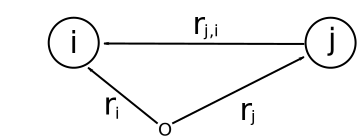
\includegraphics[width=0.5\columnwidth]{figures/vectors}
 \caption{\label{fig:md:vectors}Vectors definition between particles $i$ and $j$}
\end{figure}
%
%
Equation \eqref{eqn:md:newton} can be time integrated for every particles
$i$ using the Velocity-Verlet~(VV) scheme:
\begin{subequations}
\label{eqn:md:vv}
\begin{align}
\vx_{i}^{\pa{n+1}} & = \vx_{i}^{\pa{n}} + \vv_{i}^{\pa{n}} \Delta t +
\frac{\va_{i}^{\pa{n}}}{2} \Delta t^2, \\
\va_{i}^{\pa{n+1}} & = \frac{\vF^{\pa{n}}}{m_i}, \label{eqn:md:vv:a} \\
\vv_{i}^{\pa{n+1}} & = \vv_{i}^{\pa{n}} + \frac{\va_{i}^{\pa{n}} +
\va_{i}^{\pa{n+1}}}{2} \Delta t,
\end{align}
\end{subequations}
where $\Delta t$ is the integration time step, $\vx_{i}$ the position vector,
$\vv_{i}$ the velocity vector and $\va_{i}$ the acceleration vector, all evaluated
for particle $i$ at either the time step $n$ or the next one $n+1$.
Equations \eqref{eqn:md:vv}, when applied to every particle $i$ of the system,
can thus be used to propagate in time the whole cluster.

Every particle in the system stores its position $\vx^{\pa{n}}$, its velocity
$\vv^{\pa{n}}$ and also the total force acting on it $\vF^{\pa{n}}$. This total
force is the sum of all contribution of equation \eqref{eqn:md:coulomb:F} from
all other particles in the system.

The MD algorithm basically calculates the force between every pair of particles
in the system. Since there are $N$ total particles, there are $O\pa{N^2}$
interactions to calculate. Doubling the number of particles will quadruple the
computational burden, effectively putting an upper limit on the number of
particles that can be simulated to tens of thousands.

An example cluster can be seen on figure \ref{fig:md:cluster}.
This cluster is composed
of 147 xenon atoms (large blue spheres) and absorbs some photons (red
wave-packets) from the laser field. Atoms are ionized; electron are created
(small grey spheres) which moves through the cluster. Ions are represented with
colours going from blue for neutral to red for Xe$^{5+}$. The figure was
generated using
PyMOL\footnote{\textit{The PyMOL Molecular Graphics System}, Version 1.5.0.4,
Schrödinger, LLC. \url{http://pymol.org/}} on actual simulation-created data.


\begin{figure}
 % set opaque_background, off
 \centering
 \includegraphics[width=\figurewidth]{figures/cluster}
 \caption{\label{fig:md:cluster}Example ionized Xe$_{147}$ cluster; xenon as
          large spheres with colours from blue for neutral to full red for
          Xe$^{5+}$, electrons in small grey spheres. Photons from the laser
          field are displayed as red wave-packets.}
\end{figure}


\subsection{Short range potential shapes}
\label{section:intro:md:potentials}

\subsubsection{Potential linearity}
\label{section:intro:md:potentials:linear}

In the present work, the potential (and field) is assumed to be linear in
charge state. For example, the potential and field created by a 3+ ion will be
three times larger than the one created by a 1+ ion, for short range as for the
long range. The following close range potential derivations relies on this
property.

Additionally, the potential created by an electron is assumed to be equal in
strength but of opposite sign from the one created by a 1+ ion.

These properties greatly simplifies the case of ionization, described in chapter
\ref{section:intro:mechanisms} (page \pageref{section:intro:mechanisms}),
when a new electron is created in the code.
Indeed, when an electron is located exactly on top of an ion, right after
an ionization event for example, the resulting potential on the other particles
will have not changed.


\subsubsection{Coulomb potential singularity}
\label{section:intro:md:potentials:singularity}

An important problem to consider is the close range behaviour of the Coulomb force
in equation \eqref{eqn:md:coulomb:F} which diverges. The problem is resolved by
changing the shape of equation \eqref{eqn:md:coulomb:F} at close range.
Different \textit{smoothing potentials} can be used to prevent the
discontinuity of the Coulomb potential (or force).

Additionally, from a quantum mechanical point-of-view, electrons should not be
able to classically recombine to an ion below the ground state energy.
A softened potential also prevents the electron from falling too deep within the
potential well of an ion. If this were to happen, the cluster as a whole would
become artificially heated. However, as we will see in chapter
\ref{section:papers:100nm} (page \pageref{section:papers:100nm}), it can be
important to account for the effect of a deeper potential on a hot electron. To
account for this, and still prevent artificial cluster heating, we have
implemented electron recombination to the ground state, as described in chapter
\ref{section:intro:mechanisms} (page \pageref{section:intro:mechanisms}).

Different potential shapes were investigated for the close range potential.
Figure~\ref{fig:potential:shapes} plots the different shapes of potentials and
their respective electrostatic field. These shapes are obtained by simply
finding the location $R$ where the value and the slope of the close-range shape
$\phi_{cr}$ fits with the Coulomb potential $\phi_C$:
\begin{subequations}
\begin{align}
\left. \phi_C        \right|_{R} & = \left. \phi_{cr} \right|_{R}, \\
\left. \delr{\phi_C} \right|_{R} & = \left. \delr{\phi_{cr}} \right|_{R}.
\end{align}
\label{eqn:potential:to_match}
\end{subequations}

These locations $R$ are the cutoff radius of these shapes and mark the switch
between the long range Coulomb potential and the short range potential.


\subsubsection{Harmonic}

For the harmonic potential, we have:
\begin{align}
\phi_{j,H} & = -A r^2 + \phi_0.
\end{align}
We note that at $r_{j,i} = 0$, the potential value is the ``potential depth''
$\phi_0$.
Matching equations \eqref{eqn:potential:to_match} at $R$ gives:
\begin{subequations}
\begin{align}
\phi_{j,H}\pa{\vr_i} & = \frac{-4 \phi_0^3}{27 \pa{k q_j}^2} r_{j,i}^2 + \phi_0,
\\
R & = \frac{3 k q_j}{2 \phi_0}, \\
\vE_{j,H}\pa{\vr_i} & = \frac{k q_j}{R^3} \vr_{j,i}.
\end{align}
\end{subequations}


\subsubsection{Super-Gaussian}

The super-gaussian potential is given by:
\begin{align}
\phi_{j,SG}\pa{\vr_i} & = \phi_0 \ex{
                            -\frac{1}{2} \pa{\frac{r_{j,i}}{\sigma}}^{2m}
                        }.
\label{eqn:potential:shapes:sg:pot}
\end{align}
In the case where $m = 1$, equation \eqref{eqn:potential:shapes:sg:pot} is simply
a gaussian shape. Matching equations~\eqref{eqn:potential:to_match} at $R$ gives
values for $\sigma$ and $R$:
\begin{subequations}
\begin{align}
\sigma  & = \frac{k q_j m^{1/2m}}{\phi_0} \ex{\frac{1}{2m}}, \\
R       & = \frac{k q_j}{\phi_0} \ex{\frac{1}{2m}}, \\
\vE_{j,SG} & = \frac{\phi_0 m}{r_{j,i}}
                \ex{-\frac{1}{2} \pa{\frac{r_{j,i}}{\sigma}}^{2m}}
                \pa{ \frac{r_{j,i}}{\sigma} }^{2m}
                \hvr_{j,i}.
\end{align}
\label{eqn:potential:shapes:sg}
\end{subequations}





\subsubsection{Gaussian distribution}

An efficient way to correct the close range problem is to treat electrons as
charge distributions instead of point particles. There is thus no
discontinuity when the two charged distribution (particles) overlap. As such,
the electrostatic potential due to a charged particle $j$
(of gaussian shape of width $\sigma$) at location $\vr = r \hvr$ is
\begin{align}
\phi_{j}\pa{\vr} & = \frac{k q_j}{r} \erf{\frac{r}{\sigma \sqrt{2}}},
\label{eqn:md:smoothed:phi}
\end{align}
where $\erf{}$ is the error function. The associated electrostatic field is thus
\begin{align}
\vE_{j}\pa{\vr} & = -\grad{\phi_j\pa{\vr}} = k q_j \pa{
    \frac{ \erf{\frac{r}{\sigma\sqrt{2}}} }{r^2}
    - \sqrt{\frac{2}{\pi}} \frac{ \ex{-\frac{r^2}{2 \sigma^2}} }{\sigma r}
} \hvr.
\label{eqn:md:smoothed:E}
\end{align}
When the distance $r$ is large compared to $\sigma$, the error function
is tends towards 1 and the exponential tends towards 0 (since it's a gaussian
shape). The potential \eqref{eqn:md:smoothed:phi} and electric field
\eqref{eqn:md:smoothed:E} thus tend towards Coulombic for large distances.

The value of $\sigma$ is arbitrary: the smaller it is, the closer the potential
will be from the pure Coulomb one. We can set a value for $\sigma$ from the
extremum value of the potential which occurs at $\vr = 0$. At $\vr = 0$, an
indetermination $\frac{0}{0}$ occurs. Using l'Hospital rule, we get the limit
of $\phi$ as $\vr$ reaches 0:
\begin{align}
\lim_{\vr \rightarrow 0} \phi_j\pa{\vr}
    & \equiv \phi_j\pa{0} = \frac{ k q_j }{ \sigma } \sqrt{\frac{2}{\pi}},
\label{eqn:md:smoothed:phi0}
\end{align}
from which we get the particle width:
\begin{align}
\sigma & = \frac{ k q_j }{ \phi_j\pa{0} } \sqrt{ \frac{2}{\pi}}.
\label{eqn:md:sigma}
\end{align}
The free parameter is thus the ``potential depth'' $\phi_j\pa{0}$. Even
though $\phi_j\pa{0} > 0$ we call this parameter ``depth'' since the potential
energy of an electron on top of an ion would be minimum, similar to the
gravitational potential energy of a ball is minimum at the bottom of a well.

Another problem that the smoothing of equations \eqref{eqn:md:smoothed:phi} and
\eqref{eqn:md:smoothed:E} solve is the one of \textit{numerical heating} which
occurs when particles artificially gain (or loose) energy during the
calculation of equations \eqref{eqn:md:vv}. This absence of conservation of
energy is due to a too large time step $\Delta t$. Indeed, the
discretization of equations \eqref{eqn:md:vv}, and most importantly of
subequation \eqref{eqn:md:vv:a}, assumes the force on each particle to have a
linear variation between time steps. If the time step is too large and the
curvature of equation \eqref{eqn:md:smoothed:E} cannot be sampled by the moving
particle between each time steps, then the energy will not be conserved.



Figure \ref{fig:potential:shapes} show the different potential shapes and their
respective electrostatic field.

\begin{figure}
 \centering
 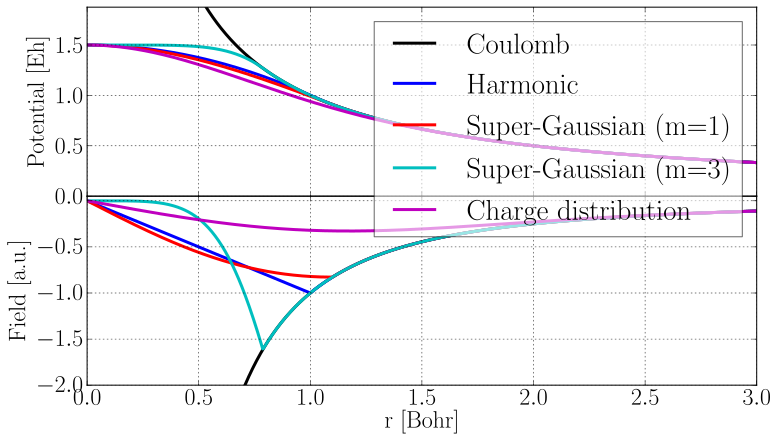
\includegraphics[width=\figurewidth]{figures/potential_shapes}
 \caption{\label{fig:potential:shapes}Potential shapes and their respective
          electric field. Note the use of atomic units and the potential depth
          $\phi_0$ = 1.5 Hartree = 40.8 eV.}
\end{figure}

It was found that the potential given by the charge distribution of equation
\eqref{eqn:md:smoothed:phi} and the associated electrostatic field of
\eqref{eqn:md:smoothed:E} give the least numerical heating. As explained
previously, the time discretization used to integrate the equations of motion
assumes that the change in force between two time steps is linear. As can be
seen on figure \ref{fig:potential:shapes}, the charge distribution curve
(magenta) does not have a discontinuity and is therefore the preferred one.

To validate the selection of the smoothing curve, photo-ionization was forced
on a single atom and the total energy calculated. In this ionization case, the
electron comes out of the ion with a maximum of kinetic energy so that
its total energy is the difference between the photon energy and the ionization
potential. It is thus a good candidate for a quantitative measurement of
numerical heating. If the total
energy is conserved, then the selected parameters (potential depth, smoothing
curve and time step) can be used with good confidence. Figures
\ref{fig:potential:heating:dt} and \ref{fig:potential:heating:depth} show the
energy variation of the process as a function of time step (for different
potential depths) and as a function of potential depth (for different time
steps). A time step of 0.5 attosecond is often taken as
it minimizes the energy variation for a large
range of potential depths, as can be seen on figure
\ref{fig:potential:heating:depth}.
It is important to note that a better precision is not obtained by going
under $\Delta~t~\approx~0.05~\textrm{as}$ as can be seen on figure
\ref{fig:potential:heating:dt}. This is caused by the precision of the computer.
While it is normal that such a limit exist, it is relatively high due to the
actual code implementation. Indeed, the dynamical aspect of the code is
implemented in SI units when large differences between numbers can be easily
obtained. When these numbers are combined in the algorithm's implementation,
the computer floating point precision is not enough. Nevertheless, a time-step
of 0.05~as is sufficient for the work. The specific
parameters (time step and potential depth) are specified in the different
studies in later chapters.

\begin{figure}
 \centering
 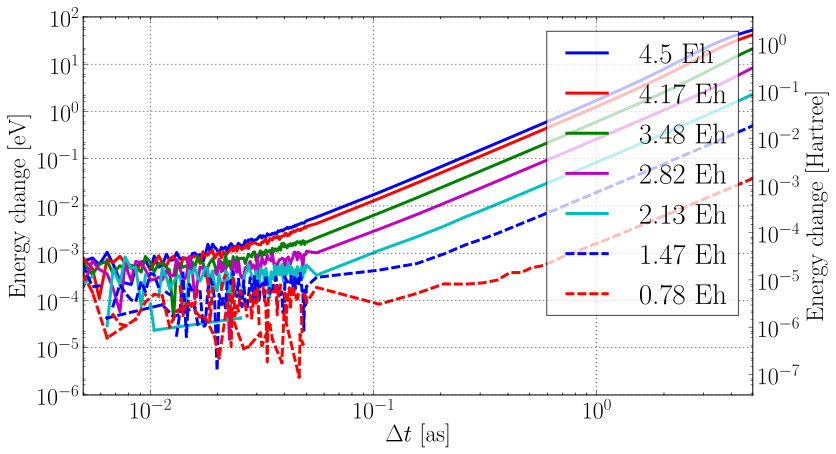
\includegraphics[width=\figurewidth]{figures/numerical_heating_dt}
 \caption{\label{fig:potential:heating:dt}Energy variation after single photon
          ionization as a function of the time step size $\Delta t$.}
\end{figure}

\begin{figure}
 \centering
 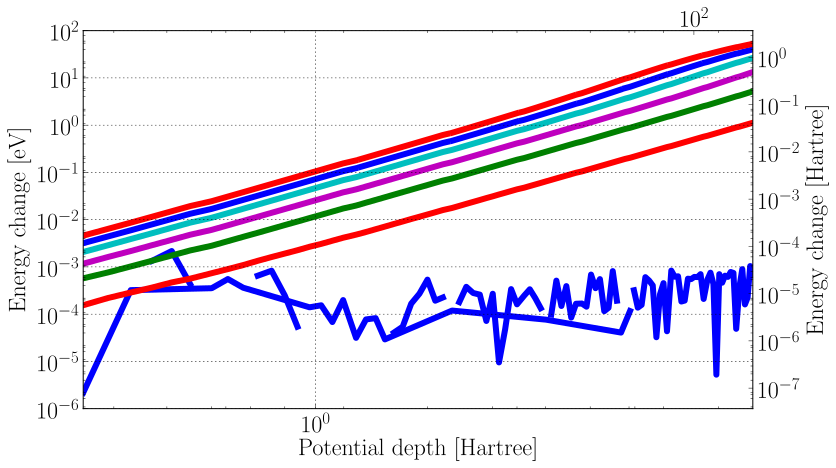
\includegraphics[width=\figurewidth]{figures/numerical_heating_D}
 \caption{\label{fig:potential:heating:depth}Energy variation after single photon
          ionization as a function of the potential depth.}
\end{figure}


\subsubsection{Look-up tables}
\label{section:intro:md:potentials:lut}

The preferred potential shape, the Gaussian distribution described previously,
uses the error function which has a major
computational issue: it is slow, or at least too slow to be called at each interaction pair
calculation. I was decided to implement a look-up table instead.
The potential and field functions are pre-calculated for a charge state of 1+.
Since both potential and field are linear in charge (the potential caused by a 2+
ion is twice the one of a 1+), their value for any
particle is simply scaled by its charge state.

Once the potential and field curves are calculated, they are approximated using
\begin{align}
x_{\textrm{norm}} & = \frac{x}{\Delta x}, \\
i   & = \textrm{int}\pa{x_{\textrm{norm}}}, \\
A   &= lut\cro{i} + \pa{lut\cro{i+1}-lut\cro{i}} \pa{x_{\textrm{norm}}-\textrm{double}\pa{i}},
\end{align}
where $x$ is the distance between the two particles, $lut$ is the array
containing the look-up table, $i$ the index of the look-up table and $A$ the
value to approximate using the look-up table.

The OpenCL implementation is different. The look-up tables are first transferred
to the OpenCL device where they will be indexed using:
\begin{align}
x_{\textrm{norm}} & = \frac{x}{\Delta x}, \\
i   & = \textrm{convert\_int\_sat\_rtz}\pa{\textrm{floor}\pa{x_{\textrm{norm}}}}, \\
A   &= lut\cro{i} + \pa{lut\cro{i+1}-lut\cro{i}} \pa{x_{\textrm{norm}}-\textrm{convert\_float}\pa{i}}.
\end{align}
The OpenCL function
convert\_float() converts an integer to a floating point value
and convert\_int\_sat\_rtz() converts a floating point to an integer,
rounding towards zero (\_rtz) and saturating (\_sat) the conversion in case of
out-of-range
\footnote{\url{https://www.khronos.org/registry/cl/sdk/1.2/docs/man/xhtml/convert_T.html}}
(if the floating point value exceed the range of the integer type,
the maximum value for the integer is used instead of a dangerous undefined
behaviour).

This effectively does a linear interpolation between the look-up table values.
In the present work, 10,000 points are used for the table with a maximum value
for $x$ at the potential shape cutoff distance. In the case of the gaussian
distribution shape, four times the particle width $\sigma$ is used as the cutoff
distance.



\subsection{Long range potential: Hierarchical Tree algorithms}
\label{section:intro:md:tree}

The $O\pa{N^2}$ scaling of the MD algorithm for long-range forces
can be problematic when the number of
particles simulated is more than many thousands, which is a potential target
for laser-cluster interaction. Some interesting variations of the MD algorithm
exist to reduce the computational burden. One class of methods uses
\textit{hierarchical tree}
algorithms as introduced by Barnes and Hut in 1986~\cite{Barnes1986}. To
reduce the computational burden, particles are grouped in a hierarchical tree
(quadtree in two dimensions, octree in three). While Barnes used his
\textit{treecode} to solve the N-body problem in the context of gravitational
interactions, it can also be applied in the electrostatic case.

The main issue with the direct calculation of forces in MD is the lack of
distinction between the close and distant particles. While the resulting
potential of a distant particle is small, the computational cost required to
calculate it is the same as in the case of a nearby particle. Some MD
calculations use an artificial cutoff: particles farther than this cutoff will
be ignored. This is acceptable
when the force acting on particles is of short range, either due to screening or
to the nature of the force (Lennard-Jones for example).
In the present work, the dominant force is the
Coulomb force and is long range by nature; it thus cannot be artificially
cut off as in the case of close range forces used in other fields.

Could distant particles be grouped together, with their contribution to the
force (or potential) being calculated only once (per ``group'')? Because
individual particles which are part of a distant group will have a similar
contribution to the potential at the location of particle $i$, the interaction
with this group can instead be approximated through the multipole
expansion~\cite{Gibbon2002} of the group of particles, or cell in terms of the
tree algorithm:
\begin{align}
\phi_i & = \sum_{j~\textrm{cell}} \phi_{j \rightarrow i} = \sum_{j~{\rm cell}}
\frac{k q_j}{r_{ji}}, \\
& \approx \frac{M_{c}}{R}
+ \sum_{\alpha} \frac{r_{\alpha} D_{c,\alpha}}{R^3}
+ \frac{1}{2} \sum_{\alpha,\beta} \frac{
        Q_{c,\alpha,\beta} r_{\alpha} r_{\beta}
    }{R^5},
\end{align}
where $M_{c}$, $D_{c,\alpha}$ and $Q_{c,\alpha,\beta}$ are the monopole, dipole
and quadrupole moments of the cell defined as:
\begin{subequations}
\begin{align}
M_{c}           ~~~~& = \sum_{j~\textrm{cell}} q_{j}, \\
D_{c,\alpha}      ~~& = \sum_{j~\textrm{cell}} q_{j} r_{j,\alpha}, \\
Q_{c,\alpha,\beta}  & = \sum_{j~\textrm{cell}} q_{j} \pa{3 r_{j,\alpha}
r_{j,\beta} - r_{j}^2} \delta_{\alpha,\beta},
\end{align}
\label{eqn:tree:moments}
\end{subequations}
and $R$ is the distance between the cell's centre-of-charge and the
particle of interest $i$.

\begin{figure}
 \centering
 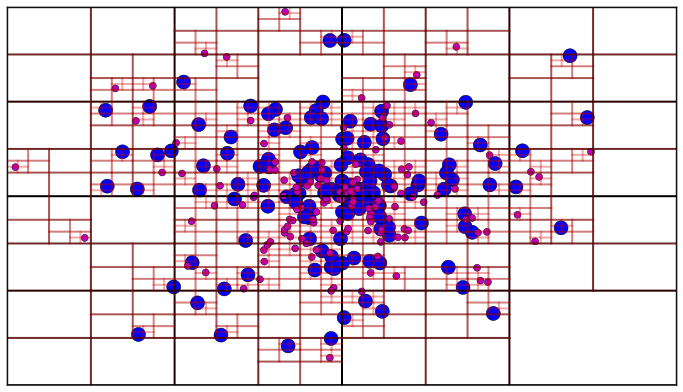
\includegraphics[width=\figurewidth]{figures/quadtree}
 \caption{\label{fig:tree:quadtree}Quadtree: 2D's equivalent of the 3D octree.
          300 particles (half ions in blue, half electrons in magenta) represent
          an exploding cluster. Cells' moments are propagated up the tree to the
          root cell. Particles distant from a cell can interact directly with it
          instead of resolving all particles contained in it, thus reducing the
          computational burden.}
\end{figure}


The tree algorithm first split the computational domain into an octree (in
three dimensions) or quadtree (in two dimensions) until
only a maximum of one particle is present per cell as can be seen figure
\ref{fig:tree:quadtree}. The deepest cells of the tree, containing only one particle,
are called leaves. Once every particle in the system is inserted in the tree,
the electrostatic moments are propagated from the leaves up to the root cell,
the top cell enclosing the whole domain.

Then, instead of iterating through all particles for the calculation of the
force on the particle of interest $i$, the tree is traversed. If the cell is
``far enough'' (with a given definition of far enough, discussed next) it can
be added to the cell interaction list for later processing through the cell's
moments. In the case of
the cell being too close, it must be resolved into its  eight \textit{daughter}
cells (or four in 2D). The daughter cells containing particles are visited, while the empty
ones are ignored. Leaf cells can be reached using this process; in this
case, the particles in the leaves are considered close enough to the particle
of interest $i$ and a direct interaction is wanted. Leaf particles will thus
be added to a second interaction list containing particle-particle direct
interactions. The process is recursively repeated until all particles
are added to an interaction list, either directly or through a parent cell.
Note that an optimization done in the
implementation allows many particles per leaves and automatically adds them
to the particles interaction list when traversing the tree, preventing trees
which are overly unbalanced.

Different selection rules exist for the criteria of ``far enough''. These
rules are called \textit{Multipole Acceptance Criteria} or
MAC~\cite{Pfalzner1996}. Barnes' original rule simply referred to as
``\textit{s/d}'' compares an input parameter $\theta$ with the cell's size $s$
divided by the distance between the cell's center-of-charge and particle of
interest $i$ (see figure \ref{fig:tree:mac:1}).
If the ratio $s/d$ is smaller than the parameter $\theta$, the
group of particles contained inside the cell is approximated through the cell's
moments and the cell is added to the cells interaction list. At the opposite, if
the ratio is larger than $\theta$, the cell will be resolved into its daughters.
In the limit where $\theta$ reaches zero, no more cells are added to the
cells interaction list (they are all resolved) and the MD algorithm emerges, though
with a large overhead due to the tree construction and traversal.

Unfortunately, this MAC can cause huge errors when a large amount of charge is
present in a corner of a cell~\cite{Pfalzner1996}.
% Page 85 (97), figure 4.13
In this case, a cell could be added to the cell
interaction list even though the error introduced by the multipole expansion is
significant. Different MAC have thus been proposed to mitigate this problem.
The \textit{minimum distance} MAC replaces the distance $d$ in the MAC with the
minimum distance to one of the cell's edge (figure \ref{fig:tree:mac:2}).
The \textit{B-max} MAC instead
replaces the size of the cell with the largest distance between one of the
cell's corner to the center-of-charge (figure \ref{fig:tree:mac:3}).
Another MAC was proposed by
B\'edorf~\textit{et.~al.}~\cite{Bedorf2012} and is a mix of the two previous.
The MAC reads:
\begin{align}
d > \frac{s}{\theta} + \delta,
\end{align}
where $\delta$ is the distance between the cell's geometric center and its
center-of-charge (figure \ref{fig:tree:mac:4}).
If the previous equation holds ($d$ is large enough) then the
multipole expansion is used and the cell is added to the interaction list.

\begin{figure}
 \centering
    \begin{subfigure}{0.15\columnwidth}
        \centering
        \includegraphics[width=\textwidth]{figures/mac_1}
        \caption{ $s/d$}
        \label{fig:tree:mac:1}
    \end{subfigure}
    \hspace{0.75cm}
    \begin{subfigure}{0.15\columnwidth}
        \centering
        \includegraphics[width=\textwidth]{figures/mac_2}
        \caption{min. $d$}
        \label{fig:tree:mac:2}
    \end{subfigure}
    \hspace{0.75cm}
    \begin{subfigure}{0.15\columnwidth}
        \centering
        \includegraphics[width=\textwidth]{figures/mac_3}
        \caption{B-max}
        \label{fig:tree:mac:3}
    \end{subfigure}
    \hspace{0.75cm}
    \begin{subfigure}{0.15\columnwidth}
        \centering
        \includegraphics[width=\textwidth]{figures/mac_4}
        \caption{Bédorf~\cite{Bedorf2012}}
        \label{fig:tree:mac:4}
    \end{subfigure}
\caption{Different Multipole Acceptance Criteria (MAC). See text for descriptions.}
\label{fig:tree:mac}
\end{figure}


Because not all interaction pairs are considered in the calculation of the
force and potential in this tree algorithm,
a significant speedup is obtained. Due to the tree
traversal algorithm, the scaling improves
from $O\pa{N^2}$ to $O\pa{N \log{N}}$~\cite{Barnes1986,Gibbon2002,Pfalzner1996}.

A variation of the hierarchical treecode is obtained when a sufficiently large
$\theta$ is used. In this case, the root cell (the largest one) is never
resolved into its daughters. By adding more moments to the approximation then
the first three of equations \eqref{eqn:tree:moments} and removing
contributions of nearby particles, the \textit{Fast Multipole Method} (FMM) is
obtained~\cite{Pfalzner1996}. FMM was developed by Greegard in
1988~\cite{Greengard1987} independently of Barnes' hierarchical tree method.
While conceptually similar, its implementation details are quite different and
it has not been implemented in the current work while the hierarchical tree
algorithm was.


\subsection{Implementation details}

The following will go over some specific details of the code implementation.
An explanation as to why a new MD code was written is first presented. The
model approximating the cluster environment for atomic processes is then
presented, followed by specific details to photon and impact ionization.
Next, the use of cross-sections for ionization events is explained and finally
recombination as implemented in the code is presented.


\subsubsection{MD code}

Our group previously used Barnes and Hut's treecode implementation,
freely available\cite{treecode} (through the GPL version 2 license). The code was adapted
to simulate charged particles (Coulomb force) instead of masses (gravitational
force) with some ionization routines added (see for example reference
\cite{Jungreuthmayer2005}). While reducing development time by re-using already
written code, the maintenance burden introduced by many factors (initial
implementation written in the C language, usage of global variables
throughout the code, multiple coding styles from different people throughout
the years, lack of revision control system giving freedom
of deleting code from the active version without losing the ability to roll
back, many subtle and important bugs, stability issues, etc.) convinced me
to start from scratch. This allowed modern development techniques to be
used. For example, all development was done through a revision control system
(subversion\cite{svn} at first, then switched to git\cite{git}) in the C++
language instead of C. The object oriented nature of C++ allowed encapsulation
of different parts of the code which could then be tested and validated
individually through unit testing. This gave much better flexibility to the
code, a required asset to
push further the development of features.

A substantial number of MD packages are freely available and
their use was considered instead of re-implementing a new one from scratch.
Examples are GROMACS\footnote{GROMACS:
\url{http://www.gromacs.org/}}, NAMD\footnote{NAMD:
\url{http://www.ks.uiuc.edu/Research/namd/}} and
LAMMPS\footnote{LAMMPS: \url{http://lammps.sandia.gov/}}. A major issue with these
pre-existing MD packages is their target audience; they aim to simulate large
bio-molecules with mostly short range interactions. Another important problem
is the number of particles throughout the simulations. While many packages
assume a constant number of particles, the present work required creating
(ionization) and annihilating (recombination) particles during simulations.
Controlling the MD part of the code allowed better integration of the
ionization aspects.

Additionally, other MD packages were not mature enough or simply non-existent at the time.
For example the largely used HOOMD-blue\footnote{HOOMD-blue:
\url{http://codeblue.umich.edu/hoomd-blue/}} which uses extensively
Nvidia GPUs released its first version (v0.6.0) in February 2008.
The knowledge and experience gained by writing from scratch such
a package is also invaluable.




\subsubsection{Potential threshold $V_b$}
\label{section:intro:Vb}

Many ionization processes described in the introduction
consider an isolated atom but
clusters have close to solid density (10$^{22}$ -- 10$^{23}$ cm$^{-3}$);
the cluster environment cannot be ignored.

This environment can be approximated by a constant value that shifts the
potential\cite{Fennel2007}. The shift is $U_b = -e_0 V_b$ where $V_b$ is the
potential due to the cluster at the ion's location (ignoring nearby electrons)
and $U_b$ is the potential energy a test particle of charge state -1 (an electron)
would have if it was placed right on top of the ion. This can be justified by
the fact that bound states of rare gas atoms are localized close to the nucleus
and the cluster potential spatial variation around atoms is small.

To illustrate this shifting, figure \ref{fig:md:Vb} shows the potential energy
landscape of an example ``cluster'' of two ions. Plotted on this figure is the
potential energy of a test particle of charge state -1 (an electron) in the
cluster environment. The contribution from the ion is the blue dashed line on the
figure. Note the distinction between potential and potential
energy. A positive charge (an ion) creates a positive potential but the
potential \textit{energy} of the test particle (of charge state -1) in that
positive potential is negative, hence the negative curves on figure
\ref{fig:md:Vb}.



\begin{figure}
    % ./potential_landscape.py --two --ion="0,1" --ion="-15,5" --impe_r=4 \
    %     --depth=1.5 --ion_impe=0 --impe_K=0.75 --ionization --umin=-1.2 \
    %     --umax=0.3 --plot=all --rmin=-7 --rmax=7.5 --plot=U
    \begin{center}
    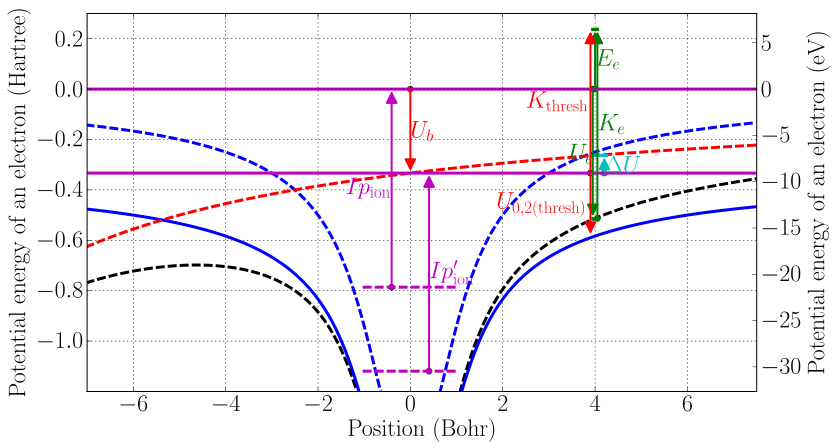
\includegraphics[width=\figurewidth]{figures/potential_landscape}
    \end{center}
    \caption{\label{fig:md:Vb}Cluster environment potential energy landscape
             and the $U_b$ approximation. A 1+ ion at $r=0$ and a 5+ at
             $r=-15$~Bohr. The potential energy curves are those of a test
             particle of charge state -1 (electron).
             The first ion's contribution is in blue-dashed line. The second ion's
             contribution is in red-dashed line and represents the cluster environment.
             The black-dashed line represents the total from the two ions.
             The blue-dotted line is the first ion's potential shifted by $U_b$.
             The upper horizontal magenta-dotted line is the isolated atom
             threshold, while the lower one is the shifted one due to the cluster
             environment.}
\end{figure}


Continuing in the example case of figure \ref{fig:md:Vb}, we introduce a
second ion as an example of the simplest cluster environment. This second ion, of
charge state 5+ in this example and located at $r$~=~-15 Bohr, is creating a
potential that is not constant around the first ion (red-dashed line). The potential energy of
the test particle in this potential is plotted as the red dashed line. The total
potential energy of the test particle due to the two ions is plotted as a black
dashed line.

The first ion's threshold is thus influenced by the second ion. The continuum,
instead of being at zero, is shifted by $U_b$. This approximates the
influence of the second ion as being constant in the first ion's vicinity. This
threshold shift is shown on figure \ref{fig:md:Vb} as the red arrow $U_b$.

The effect of $U_b$ is to shift the ion's states to lower energies. This is
shown on the figure as Ip$_{ion}$, the energy required for a bound electron
to be promoted to the isolated ion's continuum, being shifted downward to
Ip$_{ion}'$. The effective ion's potential energy curve, also shifted by $U_b$,
is shown as the dotted blue line.

This cluster potential $U_b$ is then treated as the atom's threshold
to continuum. By using $U_b$ as the threshold, atomic properties such as
impact ionization cross-sections can be used, even in the cluster environment.



\subsubsection{Notes on ionization definition}
\label{section:intro:mechanisms:notes}

Special care needs to be taken when calculating particle energies during
ionization processes. In this work, an ionization event is defined as one
electron that leaves its isolated parent ion, reaching infinity with a final
kinetic energy of zero.

As described in the previous chapter \ref{section:intro:Vb} (page
\pageref{section:intro:Vb}), the cluster
influence on ionization is approximated as a new threshold, which we call $V_b$.

The following paragraphs will discuss some specific details concerning single
photon ionization and impact ionization, both in the special case of an isolated
atom or ion. The generalization to the cluster environment is done through the
updated threshold, as discussed in chapter \ref{section:intro:Vb} (page
\pageref{section:intro:Vb}).


\subsubsubsection{Single photon ionization}

In the case of single photon ionization, a new electron is created right on top
of the ion with an updated charge state. At this point, all other particles in
the cluster will not see a difference; the potential $\phi'\pa{\vr}$ created by
this new particles pair
\begin{align}
\phi'\pa{\vr} & = \phi_{j}\pa{\vr;Z+1} + \phi_{k}\pa{\vr;-1},
\end{align}
is the same as the previous ion's $\phi_{j}\pa{\vr;Z}$ (see equation
\eqref{eqn:md:smoothed:phi} for the potential shape mainly used).


For the new electron to reach infinity with a null kinetic energy, it
must have, at its creation time, enough kinetic energy to leave the ion. This
kinetic energy must thus match the potential energy between the ion (with an
updated charge state) and the electron so the total energy of the electron with
respect to the ion is zero.

Additionally, the electron will contain in its kinetic energy the difference
between the absorbed photon and the ionization potential of the ion.


\subsubsubsection{Impact ionization}

For impact ionization (still in the case of an isolated atom),
the impacting electron's kinetic energy used in equation
\eqref{eqn:impact:ionization:lotz} is the kinetic energy the electron has
\textit{at infinity}, meaning that the impacting electron and the isolated
atom (or ion) are separated in an unbound system.

At infinity, the electron's total energy only contains kinetic
energy. We call this kinetic energy $K_{\textrm{thresh}}$ for ``kinetic energy
above the threshold''. This $K_{\textrm{thresh}}$ can simply be calculated
as $K_{\textrm{thresh}} = \textrm{max}\pa{0, K_e + U_e}$
where $K_e$ is the
electron's kinetic energy and $U_e$ its potential energy with respect to the ion.
$K_{\textrm{thresh}}$ is thus the electron's total energy \textit{with respect
to the ion}.
In the case of a classically bound electron, the total energy is less than zero:
the max() enforces a positive kinetic energy.

When a cluster environment is present, a similar approach is taken to obtain
$K_{\textrm{thresh}}$. Instead of taking the extra energy above zero for
$K_{\textrm{thresh}}$, the extra energy above the new threshold $U_b$ is used.
This value can easily be obtained from the actual electron's kinetic energy
$K_e$, it's \textit{total} potential energy in the cluster environment and the
threshold $U_b$ by:
\begin{align}
K_{\textrm{thresh}} & = \textrm{max}\pa{0, K_e + U_e - U_b}
\label{eqn:md:kthresh}
\end{align}
and is shown on figure \ref{fig:md:Vb} as a red arrow with its base at $U_b$.


$K_{\textrm{thresh}}$ is the kinetic energy that must be used in Lotz formula
\eqref{eqn:impact:ionization:lotz}. Cross-sections are discussed in the next
section.


When an impact ionization event occurs and if the impacting electron has more kinetic
energy, it can either keep the extra, give all the extra, or give a fraction of
the extra to the new electron. We split the extra kinetic energy between the two
electrons to assure that they do not fall back into the ion.


% Figure \ref{fig:impact:before:Z} shows the process of impact ionization when an
% electron (particle 1) of charge state -1 impacts an ion (particle 0) of charge
% state Z and creates a new electron (particle 2) right on top.
%
% \begin{figure}
%  \centering
%     \begin{subfigure}{0.48\columnwidth}
%         \centering
%         \includegraphics[width=\textwidth]{figures/impact_ionization_t00}
%         \caption{Before impact ionization (Z)}
%         \label{fig:impact:before:Z}
%     \end{subfigure}
% \\
%     \begin{subfigure}{0.48\columnwidth}
%         \centering
%         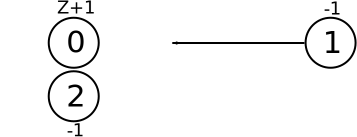
\includegraphics[width=\textwidth]{figures/impact_ionization_t0}
%         \caption{During impact ionization (Z+1)}
%         \label{fig:impact:before:Zp1}
%     \end{subfigure}
% %
%     \begin{subfigure}{0.48\columnwidth}
%         \centering
%         \includegraphics[width=\textwidth]{figures/impact_ionization_t1}
%         \caption{After impact ionization}
%         \label{fig:impact:after}
%     \end{subfigure}
% \caption{Impact ionization: before and after}
% \label{fig:impact:steps}
% \end{figure}


% First, let's assume the impacting electron came from infinity where it's kinetic
% energy was exactly the Ip. In that case, impact ionization will occur (considering
% its impact parameter lies inside the cross-section). By definition, we must have two
% electrons leaving to infinity: an unbound system. Such an unbound system has a total
% energy of 0.
%
% The total energy before (a) is thus:
% \begin{align}
% E^{a} & = K_{1}^{a} + U_{01}^{a} = Ip
% \label{eqn:Ea}
% \end{align}
% and after (c) ionization is:
% \begin{align}
% E^{c} & = K_{1}^{c} + K_{2}^{c} + U_{01}^{c} + U_{02}^{c} + U_{12}^{c} = 0
% \label{eqn:Ec}
% \end{align}
%
% The change in energy is thus:
% \begin{align}
% E^{a} - E^{c} & = Ip = K_{1}^{a} + U_{01}^{a} - \pa{
%     K_{1}^{c} + K_{2}^{c} + U_{01}^{c} + U_{02}^{c} + U_{12}^{c}
% }
% \end{align}
%
% The only unknown values here are $K_{1}^{c}$ and $K_{2}^{c}$ since the new electron is
% created right on top of the ion. Let's isolate the final kinetic energies:
% \begin{align}
% K_{1}^{c} + K_{2}^{c} = K_{1}^{a} + U_{01}^{a} - \pa{
%     U_{01}^{c} + U_{02}^{c} + U_{12}^{c}
% } - Ip
% \label{eqn:K1cPlusK2c}
% \end{align}
%
% We have a single constraint from equation \eqref{eqn:K1cPlusK2c} but two unknown. We thus
% give an arbitrary value to one of the two. We want the new electron to leave the ion.
% Since it is right on top of it, we can guess the required kinetic energy to be very close
% to (minus) the potential energy the electron has with respect to the ion. But this electron
% will be ``pushed'' be the impacting electron too and will thus be accelerated. To compensate
% for this push, we remove the potential energy between the two electrons from the new electron's
% kinetic energy. So the educated guess for the final kinetic energy of the new electron is:
% \begin{align}
% K_{2}^{c} & = -U_{02}^{c} - U_{12}^{c}
% \label{eqn:K2c:pushed}
% \end{align}
%
% Using equation \eqref{eqn:K2c:pushed} in equation \eqref{eqn:K1cPlusK2c} gives:
% \begin{align}
% K_{1}^{c}
%  & = K_{1}^{a} + U_{01}^{a} - \pa{
%     U_{01}^{c} + U_{02}^{c} + U_{12}^{c}
% } - Ip - K_{2}^{c} \\
%  & = K_{1}^{a} + U_{01}^{a} - \pa{
%     U_{01}^{c} + \cancel{ U_{02}^{c} } + \bcancel{ U_{12}^{c} }
% } - Ip + \cancel{ U_{02}^{c} } + \bcancel{ U_{12}^{c} } \\
% K_{1}^{c}
%  & = K_{1}^{a} + U_{01}^{a} - U_{01}^{c} - Ip
% \label{eqn:K1c:pushed}
% \end{align}
%
% The final total energy is then:
% \begin{align}
% E^{c}
%  & = \pa{
%     K_{1}^{a} + U_{01}^{a} - \cancel{ U_{01}^{c} } - Ip
%  } - \pa{
%                  \cancel{ U_{02}^{c} } + \bcancel{ U_{12}^{c} }
% } + \cancel{ U_{01}^{c} } + \cancel{ U_{02}^{c} } + \bcancel{ U_{12}^{c} } \\
%  & = K_{1}^{a} + U_{01}^{a} - Ip \\
%  & = Ip - Ip \\
% E^{c} & = 0
% \end{align}
% which is what was expected.






% Additionally, momentum is conserved by giving the two leaving electrons an angle
% of divergence. Since the impacting electron can cause ionization before being
% exactly on top of the atom or ion, the angle of divergence is given by:
%
% Figure \ref{fig:impact:direction} shows the convention of the two angles $\theta$ and $\phi$.
%
% \begin{figure}
% \begin{center}
% \includegraphics[width=0.8\textwidth]{figures/impact_ionization_directions}
% \end{center}
% \caption{Impact ionization: Direction for electrons}
% \label{fig:impact:direction}
% \end{figure}
%
%
% Momentum is conserved in each dimension. In this case, it's a 2-D plane.
% \begin{align}
% \vp^{a} & = \vp^{c} \\
% \vp^{a} & = m_e v_{1x}^{a} \hat{x} \\
% \vp^{c} & = m_e \pa{v_{1x}^{c} + v_{2x}^{c}} \hat{x} + m_e \pa{v_{1y}^{c} + v_{2y}^{c}} \hat{y}
% \end{align}
% with:
% \begin{subequations}
% \begin{align}
% v_{1x}^{a} & =  v_{1}^{a} \\
% v_{1x}^{c} & =  v_{1}^{c} \cosine{\theta} \\
% v_{2x}^{c} & =  v_{2}^{c} \cosine{\phi} \\
% v_{1y}^{c} & =  v_{1}^{c} \sine{\theta} \\
% v_{2y}^{c} & = -v_{2}^{c} \sine{\phi}
% \end{align}
% \end{subequations}
%
% Conservation in $x$:
% \begin{align}
% v_{1x}^{a}      & = v_{1x}^{c} + v_{2x}^{c} \\
% v_{1}^{a}       & = v_{1}^{c} \cosine{\theta} + v_{2}^{c} \cosine{\phi} \\
% \cosine{\phi}   & = \frac{v_{1}^{a} - v_{1}^{c} \cosine{\theta}}{v_{2}^{c}}
% \label{eqn:cos_phi}
% \end{align}
% and in $y$:
% \begin{align}
% 0           & = v_{1y}^{c} + v_{2y}^{c} \\
% 0           & = v_{1}^{c} \sine{\theta} - v_{2}^{c} \sine{\phi} \\
% \sine{\phi} & = \frac{v_{1}^{c}}{v_{2}^{c}} \sine{\theta}
% \label{eqn:sin_phi}
%  % \\
% % \phi        & = \asin{ \frac{v_{1}^{c}}{v_{2}^{c}} \sine{\theta} }
% \end{align}
%
% Squaring and summing \eqref{eqn:cos_phi} and \eqref{eqn:sin_phi} gives 1:
% \begin{align}
% 1
% & = \cossquared{\phi} + \sinsquared{\phi} \\
% & = \pa{ \frac{v_{1}^{a} - v_{1}^{c} \cosine{\theta}}{v_{2}^{c}} }^2
%   + \pa{ \frac{v_{1}^{c}}{v_{2}^{c}} \sine{\theta} }^{2} \\
% \pa{ v_{2}^{c} }^2
% & = \pa{ v_{1}^{a} - v_{1}^{c} \cosine{\theta} }^2
%   + \pa{ v_{1}^{c} \sine{\theta} }^{2} \\
% & = \pa{ v_{1}^{a} }^{2} + \pa{ v_{1}^{c} }^{2} \cossquared{\theta}
%     - 2 v_{1}^{a} v_{1}^{c} \cosine{\theta}
%     + \pa{ v_{1}^{c} }^{2} \sinsquared{\theta} \\
% & =   \pa{ v_{1}^{c} }^{2} \underbrace{\pa{ \cossquared{\theta} + \sinsquared{\theta} }}_{=1}
%     + \pa{ v_{1}^{a} }^{2}
%     - 2 v_{1}^{a} v_{1}^{c} \cosine{\theta} \\
% \pa{ v_{2}^{c} }^2
% & =   \pa{ v_{1}^{c} }^{2}
%     + \pa{ v_{1}^{a} }^{2}
%     - 2 v_{1}^{a} v_{1}^{c} \cosine{\theta} \\
% 2 v_{1}^{a} v_{1}^{c} \cosine{\theta}
% & =   \pa{ v_{1}^{c} }^{2}
%     + \pa{ v_{1}^{a} }^{2}
%     - \pa{ v_{2}^{c} }^2 \\
% \cosine{\theta}
% & = \frac{
%       \pa{ v_{1}^{a} }^{2}
%     + \pa{ v_{1}^{c} }^{2}
%     - \pa{ v_{2}^{c} }^2
%     }{ 2 v_{1}^{a} v_{1}^{c} }
% \label{eqn:cos_theta}
% \end{align}
%
% Equation \eqref{eqn:cos_theta} is used to get $\theta$ from $v_{1}^{a}$ (initial velocity of
% the impacting electron), $v_{1}^{c}$ (final velocity of the impacting electron) and
% $v_{2}^{c}$ (final velocity of new electron). Once the angle $\theta$ is found, $\phi$ can
% be found using \eqref{eqn:cos_phi}.
%



\subsubsection{Cross-sections}
\label{section:intro:md:cross-sections}

Implementing any kind of ionization in the model is done through cross-sections.
Because cross-sections can be obtained from experiments for any kind of target,
it is easily integrated into the model.

\subsubsubsection{Single photon ionization}

For single-photon ionization, experimental cross-sections $\sigma\pa{\omega}$
for xenon were obtained from reference \cite{West1978} and from
reference \cite{Marr1976} for argon.

Once cross-sections are obtained, they are converted to a rate of ionization
using
\begin{align}
\Gamma\pa{\omega} = \sigma\pa{\omega} I\pa{t}.
\label{eqn:ionization:rate:single}
\end{align}
which is equivalent to equation \eqref{eqn:ionization:rate:mpi} with $\nu = 1$.

Then, this rate is weighted\cite{Lax2006} by the time step size and compared to
a random number $r$ between 0 and 1:
\begin{align}
1 - \e{-\Gamma \Delta t} > r.
\label{eqn:ionization:prob}
\end{align}
When the previous test succeeds, ionization takes place and a new electron is
created in the code.
Then, the intensity profile of the laser $I\pa{t}$ is decreased
by one photon
%
to incorporate laser depletion. This is especially important
for a more accurate description of cluster interaction with low fluence pulses.


\subsubsubsection{Collisional processes}

For impact ionization cross-sections, Lotz formula of equation
\eqref{eqn:impact:ionization:lotz} is used with experimental parameters obtained
from reference \cite{Tawara1987} (for neutral xenon)
% Figure 254, page 317
and \cite{Heidenreich2005} (for higher charge states).
% Parameters were taken from figure 1 (a), (b) and (c)
% Note that parameters from figure 1 (a) and (b) for
% the 4+ and 5+ do not give satisfactory results. They were
% obtained by fitting the data directly from the figures
For argon, data from \cite{Lotz1967} and \cite{Lotz1970} is used.
When $K_{\textrm{thresh}} \le 0$, a null cross-section is simply used.

As for ACI, numerical cross-sections from ground state to excited state and from
excited state to continuum were calculated by Edward Ackad using a
Hartree-Fock code from Cowan\cite{Cowan1981,CowanCode}. Only the first eight excited states
were considered (with $l<4$) for charge states up to 17+ for both xenon and argon.

The impact parameter of the impacting electron is calculated by:
\begin{align}
b & = \frac{\abs{\vv \times \vr}}{\abs{\vv}},
\label{eqn:ionization:impact:parameter}
\end{align}
where $\vv$ is the impacting electron's velocity vector and $\vr$ the vector
from the impacting electron to the target. If the impacting parameter lies
inside the calculated cross-section, excitation or ionization takes place. In
the case of excitation, the total cross-section of all excited states are used
and a final state randomly selected between all accessible, weighted by their
cross-sections relative to the total one.

% http://en.wikipedia.org/wiki/Neutron_cross_section#Link_to_reaction_rate_and_interpretation

\subsubsection{Recombination}

In a classical simulation electrons could cool down into the ions' infinite Coulomb
potential where they would have a total energy less than what is allowed
according to quantum mechanics. This would lead to artificial cluster heating,
as this electron gives up its energy to the cluster as it cools.
Using a smoothing potential as in equation
\eqref{eqn:md:smoothed:phi} will prevent the singularity.
Additionally, if the potential depth $\phi\pa{0}$ used (see
equation \eqref{eqn:md:smoothed:phi0}) is deep enough, the total energy of an
electron might fall below the energy of the state.
Recombination to the ground state is thus used to prevent such nonphysical events.
When an electron's total energy (with respect to the ion) falls below the energy
of the lowest unoccupied state,
recombination is forced: the electron disappears from the simulation and the ion
charge state is decreased by one.

Additionally, recombination plays an important role in the dynamics of the
exploding cluster. Experiments at FLASH in 2009 on xenon clusters in the XUV
regime\cite{Thomas2009} could be reproduced by our models when recombination
was enabled; we found that the lower charge states detected would come from the
cluster core where recombination is important. This study was published in
May 2013's edition of \textit{New Journal of Physics}\cite{Ackad2013} and is
included in this thesis in chapter \ref{section:papers:recomb}
(page \pageref{section:papers:recomb}).

Recombination was also required for the work in chapter
\ref{section:papers:100nm} (page \pageref{section:papers:100nm}),
as it allowed us to lower the potential depth of the
ions for more physical simulations.


\input{chapter_2p5_qfdtd}
\subsection{Acceleration through video cards and OpenCL}
\label{section:tools:opencl}

A new trend in High Performance Computing (HPC) is code acceleration
through graphics cards. Similar to the ubiquitous Moore's Law in the CPU world,
video cards power evolved exponentially during the last twenty years, pushed
by the never ending need of more realistic video games. From ``dumb'' devices
drawing primitive shapes on a display, they evolved to extremely powerful
devices and started to act more like CPUs by being programmable (shaders) during
the first half decade  of 2000. The term \textit{Graphical Processing Unit} (GPU) was
coined in 1999 by Nvidia, the biggest vendor of video cards, as a selling point
for their product and to emphasize the fact that their chips were becoming more
and more like CPUs.


\subsubsection{General-Programming GPU (GP-GPU)}

Due to this increase in power, attempts were made to use these video cards as
accelerators for computations other than real video operations. Because GPUs have
intrinsically high parallelism (for example the same operation is performed on
all pixels of an image in parallel) HPC users and developers became interested.
In his 2005 book, Taflove described a way to use a video card's GPU to
accelerate his electrodynamics FDTD solver~\cite{Taflove2005}. At that time no
General-Programming GPU (GP-GPU) framework existed so Taflove (and anyone
interested in using GPUs at that time) had to ``translate'' the FDTD algorithm
into one that could be understood by a video card. This process was extremely
difficult as it required using low level graphic primitives; in his case, OpenGL
calls.
Normally OpenGL, the Open Graphics Library,
is used to draw animated scenes on the user's screen; it must not be confused
with OpenCL described later.
A notable example of OpenGL usage is video games where the user is immersed in a
virtual three dimensional space. The process of re-writing an algorithm into
OpenGL calls is one that only a few highly skilled and knowledgeable people can
tackle.

In 2007, Nvidia saw an opportunity for market expansion. Why not let
the non-videogames programmer use the powerful GPUs for something other than video
operations? For this to happen, a programming framework had to be released; the
number of programmers and scientists able to exploit OpenGL to their advantage
was limited. They thus released their \textit{Compute Unified Device
Architecture}, later renamed CUDA.
CUDA allows writing normal C or
C++ programs with some extensions, called \textit{kernels}, that can be run on
the GPU. These kernels have the same structure as C functions but are executed
concurrently by every core on the GPU\footnote{Technically, GPUs don't have
``cores'' \textit{per se} like CPUs but the comparison can still be made.}. The
number of cores on a recent consumer grade video card is now of the order of
many hundreds; a 50\$ Nvidia GT 620 has 96 CUDA cores and 1 GB of RAM, while the
GTX TITAN has 2688 CUDA cores and 6 GB but costs more than 1,000 \$. Even though
the highest priced GPU can be more expensive than complete workstations, no CPUs
can offer close to three thousand cores for a still affordable price.

A year after CUDA was released, Apple wanted a framework that would allow
programs to be accelerated on their top-of-the-line product's GPU while still
being able to run on their lower-end range of products (which did not have a
discrete video card). Additionally, some Apple products were released with ATI
video cards (Nvidia's main competitor) which, understandably, never supported
CUDA. They thus released a framework called \textit{OpenCL} (standing for
Open Compute Language) in 2008 with the help of many partners (IBM, ATI, Intel
and even Nvidia). While conceptually similar to CUDA (smaller routines are
written in a kernel function and launched individually on the GPUs by the main
program) OpenCL has the advantage of targeting heterogeneous platforms
consisting of (possibly and not limited to) many CPUs, many cores and GPUs. The
main advantage of OpenCL is its portability; a program written in OpenCL can
not only run on GPUs from ATI and Nvidia but also on traditional CPUs,
exploiting all cores available on the CPUs transparently.

It was thus decided to port the two codes (MD and QFDTD) to OpenCL to take
advantage of the GPU power while retaining portability.


\subsubsection{GPU programming challenges}

Porting a code to run on GPUs is not as simple as recompiling
for the new architecture. While being portable, OpenCL does require, unfortunately, rewriting
many parts of the code.


\subsubsubsection{Refactoring}

Certain factors must be considered when porting codes to GPU frameworks.
First, because GPU cores are much slower than a core on a CPU,
parallelisms must be extracted from algorithms. The code must thus be
completely refactored to exploit the parallelism. For example, a CPU
implementation of the MD algorithm can be implemented by looping over particles
and calculating all properties at once, for every particle. On the contrary,
due to the high vectorized nature of GPUs, it makes more sense to calculate
only one particle property but for all particles before switching to the next
property.

Second, the main drawback of
GP-GPU programming is the fact that GPUs have their own memory, independent of
the system's memory; kernels will only have access to the device's memory. Data
required for kernel calculation must thus be first transferred to the device's
memory and similarly the resulting data must be transferred back to the host
memory where it can be further processed by the rest of the main program. Video
cards today are connected to a computer through PCI-Express (PCIe) connections.
While fast, there can still be a bottleneck if data is to be transferred back and
forth similarly to main memory. It is thus necessary to reduce to a minimum the
data transfer between the host and the device, similarly to communications in a
distributed memory parallel programming paradigm.

In the case of the MD algorithm, every interaction pair is independent of all
others and can thus be calculated concurrently; this is the basis of the
OpenCL implementation. The main loop that calculates the electrostatic field
and potential at every particle's position is implemented as an OpenCL kernel.
Each thread on the GPU will thus calculate the interaction between one particle
and all others. Once the MD kernels are launched on the GPU; they are only
halted when either the ionization routines have to be called (every femtosecond) or
when data needs to be saved (to take a snapshot of the simulation for example).
This prevents the GPU from being interrupted too often and reduces the amount of
data transfers. Using this OpenCL implementation, MD simulations could be run
80 times faster on GPUs than on conventional CPUs.

As for the QFDTD, only the real time algorithm was implemented as OpenCL
kernels since the imaginary time method did not require long simulation times.
As in the case of the MD, the real time algorithm is left running on the GPU
until data needs to be saved to a snapshot or post-processed to reduce
transfers.



\subsubsubsection{Debugging}

One of the most problematic aspects of GPU programming is the lack of debugging
tools. Many tools and techniques exist to detect and fix problems in
normal CPU codes. The following describes them and their counterpart, when present,
on GPUs.


\subsubsubsubsection{Printing}

The simplest case of debugging is printing the variables' values to the screen
and inspecting them for
erroneous values. While not really efficient, it is sometimes useful, quick
and simple ``hack'' to get an insight of how the code is working. Unfortunately,
such printing function (such as C or C++'s \textit{printf()}) cannot be used at
all on a GPU! The reason is that the main processor must be able to
\textit{read} the variable from memory to be able to print it to screen and yet
the variable's content is \textit{not} in main memory, only the video card's
memory. It must be noted though that some OpenCL drivers (for example AMD's
APP SDK\footnote{\url{http://developer.amd.com/tools-and-sdks/heterogeneous-computing/amd-accelerated-parallel-processing-app-sdk/}}
or Intel's SDK for OpenCL Applications
2013\footnote{\url{http://software.intel.com/en-us/vcsource/tools/opencl-sdk}})
have specific extensions that allow using \textit{printf()}-like functions
inside OpenCL kernels. These extensions must explicitly be enabled in kernel
files using
\begin{verbatim}
    #pragma OPENCL EXTENSION cl_amd_printf : enable
\end{verbatim}
for the Intel SDK, or
\begin{verbatim}
    #pragma OPENCL EXTENSION cl_intel_printf : enable
\end{verbatim}
for the AMD SDK. These extensions are possible since these drivers support
running the kernels directly on the CPU. In the case of AMD, the extension only
works when the kernel are executed on the CPU (not on an AMD video card). Nvidia
does not have a similar extension for their OpenCL driver. Debugging using
printf() is thus easier when running on a CPU with either Intel's or AMD SDK.


\subsubsubsubsection{Valgrind}
\label{section:tools:opencl:valgrind}

Another useful bug squashing weapon used in debugging on Linux is called
\textit{valgrind}\footnote{\url{http://www.valgrind.org/}}. This extremely
useful tool verifies memory access and can thus report on out-of-bound accesses
(accessing memory locations which are out of range of an array), a major
type of error in programming that one \textit{has} to expect to happen.
Valgrind can also detect uses of uninitialized variables, a dangerous type of
error that can be hard to detect otherwise.

Since valgrind was specifically designed to intercept main memory access it
cannot be used when the program is running of a GPU. Alternatively, when the
program is running on the CPU through the use of the Intel or AMD SDKs, valgrind
detects a huge amount of errors, probably due to errors \textit{inside} these
SDKs, rendering the analysis useless.

One of the best tool in debugging code cannot, unfortunately, be used to debug
codes running on GPUs.


\subsubsubsubsection{Debuggers}

The last tool used in debugging is an actual debugger. A normal debugger will
take control of the program, allowing the developer to pause the execution
at any time, inspect variables' values or even change them. A popular debugger
on Linux is the free and open-source \textit{gdb}, the GNU Project
debugger\footnote{\url{https://www.gnu.org/software/gdb/}}. Many more
proprietary debuggers exist, some of them free and others expensive. Traditional
debuggers work by taking control of the program and accessing
directly their memory content. It is not possible for them to access GPU memory
or control functions inside the different SDKs. Some debuggers, like
the pricey but powerful DDT\footnote{\url{http://www.allinea.com/products/ddt/}}
allow some form of debugging capabilities on video cards. A free one
called gDEBugger\footnote{\url{http://www.gremedy.com/}} supported
debugging OpenCL kernels. It was acquired by AMD which released an updated
version\footnote{\url{http://developer.amd.com/tools-and-sdks/heterogeneous-computing/amd-gdebugger/}}
in April 2012 but discontinued it. It was superseded by
CodeXL\footnote{\url{http://developer.amd.com/tools-and-sdks/heterogeneous-computing/codexl/}}
released in February 2013. As can be seen, at the time of the code was developed
the different debuggers available were scarce, limited or expensive but are now
maturing.


\subsubsubsection{HPC Facilities}

While high performance computing (HPC) are relatively widespread and accessible,
GPU clusters are harder to find.
SHARCNET\footnote{\url{https://www.sharcnet.ca/}}, a large HPC
consortium, has two clusters containing GPUs (Angel and Monk) but they are
obviously submerged by user demand.

Prof. Thomas Brabec and my supervisor Prof. Lora Ramunno were able to purchase
a GPU cluster, spurring the development of the GPU codes described above.

Due to my experience with GPUs, I was placed in charge of the purchase process
which consisted in building a solution that would maximize the performance
while staying under-budget, communicating with multiple vendors to validate
the solution, writing a Request for Proposals (RFP) and transparently evaluating
vendors offering. Additionally, I (remotely) installed and configured the
operating system (Gentoo Linux\footnote{\url{http://www.gentoo.org/}}) before
the equipment was shipped in August 2012 and also configured the queuing system
(Slurm\footnote{\url{http://www.schedmd.com}}) to maximize the cluster's
resources and even submitting new
features\footnote{\url{http://slurm.schedmd.com/team.html}}.

This HPC cluster (Primus), containing 20 Nvidia Tesla M2075 video cards, is an important
lab component that will be allow the research group to continue its high profile
research.




\input{chapter_2p7_libraries}


\fxfatal{Should it be ``Xenon'' or ``xenon''? Same for Argon, Nitrogen, Neon and Helium.}
\fxnote{Add comma after equations as they are part of the sentence.}

% Papers here
\include{chapter_3_paper_1_aci}
\include{paper_2_size}

\newcommand{\PaperTitleHundrednm}{Augmented Collisional Ionization in the VUV regime; a theoretical study}

\section{\PaperTitleHundrednm}
\label{section:papers:100nm}

\begin{flushright}
Nicolas Bigaouette, Edward Ackad, Lora Ramunno\\
To be published
\end{flushright}

% Include PDF's abstract in the Table-of-Content as ``subsection 0'' but hide the number
\HidePDFAbstractNumber

\subsection{Author contributions}
The MD package was mostly written by N. B. The ACI cross-sections were calculated
by E. A. All post processing scripts used to analyze data and generate figures
were written by N. B. Data generation and analysis was performed by N. B.
All authors contributed to the discussion.


\includepdf[pages=-,
            addtotoc={
                % Original PDF page, TOC Section hierarchy, # matching TOC level, TOC label, \label{}
                % http://cs.brown.edu/system/software/latex/doc/pdfpages.pdf
                1,subsection,2,Abstract,paper_100nm_abstract,
                1,subsection,2,Introduction,paper_100nm_intro,
                2,subsection,2,Model,paper_100nm_model,
                2,subsubsection,3,Threshold,paper_100nm_thresh,
                2,subsubsection,3,Heating Mechanisms,paper_100nm_heating,
                3,paragraph,4,Single photon ionization,paper_100nm_single,
                3,paragraph,4,Impact ionization,paper_100nm_impact,
                3,paragraph,4,Excited States (ACI),paper_100nm_aci,
                3,subsubsection,3,Recombination,paper_100nm_recomb,
                3,subsubsection,3,Many Body Recombination,paper_100nm_mbr,
                4,subsection,2,Results,paper_100nm_results,
                4,subsubsection,3,Model validation,paper_100nm_results_val,
                5,subsubsection,3,Revisiting the 100nm experiment,paper_100nm_results_100nm,
                6,subsubsection,3,Deeper potential,paper_100nm_results_deeper,
                7,subsection,2,Conclusion,paper_100nm_results_conc,
                8,subsection,2,References,paper_100nm_results_refs
            }]{papers/Bigaouette2013_100nm.pdf}

\include{paper_4_recomb}
\include{paper_5_mapping}

% \section{Other contributions}

\lipsum[1]



\section{Conclusion}

Clusters of atoms are without a doubt an extremely useful tool to study
laser and matter interaction. They were in used even before atoms were discovered
for their optical properties. With the advancement of both clusters creation
and laser technologies, it became possible to gain a significant understanding
on how light interacts with matter. Clusters studies thus became an important
physics research area.

At the simplest level, quantum mechanic describes the dynamics but exact solutions
are not possible for systems of more than two electrons.
The process of photo-ionization of single atoms is known, but the high density
of atoms inside clusters gives rise to interesting phenomena. It was a surprise
to scientists ten years ago to see highly charged ions coming out of experiments
using rare gas clusters with short duration (tens of femtoseconds), high intensity
(10$^{12}$ -- 10$^{14}$ W/cm$^2$) and small wavelength (VUV, XUV) laser pulses.
More than ten years later, our understanding of the different mechanisms of energy
absorption and diffusion throughout the cluster is taking shape. Even though full
quantum mechanical description of clusters is not possible, small approximations
can be taken, allowing theoretical and numerical studies to be performed.

Our numerical tool of choice is Molecular Dynamics where we track, classically,
the dynamics of electrons and ions during and after a laser pulse. MD simulations,
being classical systems, allows a larger number of particles than full quantum
simulations but can still describe the large fluctuations in charge and field
generated inside a cluster.

Many different MD packages are available freely that could have been used for
the current work. After a first try with one such package, it was decided to
start from scratch a new one. The MD algorithm is relatively simple; having
control on the rest of the package allowed flexibility in the development that
would have not been possible with a third party package. Fore example, existing
MD codes have specific target users that don't have the same requirements as what
was required for this work such as varying number of particles during the
simulation or long range interactions. By building the tools myself I was able
to have more trust in it by subjecting it to rigorous tests and validations.
Additionally, even though a lot of work was put into the creation of this code
base, much time was saved trying to understand or even worst, debug, code from
someone else. Having known at first the amount of time lost on an unstable code
base I would have started my MD package right away as it proved a lot easier
to move forward with it.


The $O(N^2)$ scaling of the MD algorithm prevents simulations of more than tens
of thousands of particles but interesting results are still accessible.

For bigger systems, some algorithm changes can be done to speed the force
calculation on particles. Using a hierarchical tree can change the algorithm
scaling from $O(N^2)$ to $O(N \textrm{log}\pa{N})$ and thus push the limit on
cluster size upward. Having control and full understanding of the code had
the added benefit of easing the process of adding new feature. While the tree
algorithm is implemented, it was not yet used in a publication. An interesting
technology matured during the last decade; by running codes directly on GP-GPUs,
the same algorithms could perform up to one hundred times faster than on
conventional CPUs. The MD package was thus ported to the framework OpenCL where
the MD algorithm shown a speedup of close to 80. This implementation was used
mainly in our publications since the cluster sizes we were interested in were
in the range accessible through MD (and not requiring the tree). The
hierarchical tree-based algorithm is still accessible through an input parameter
(not as an OpenCL implementation though), making the MD package interesting for
future studies where larger clusters will be investigated.

In our first publication in 2011, Edward Ackad, Lora Ramunno and I introduced
the new concept of excited states as a multi-step process of energy transfer
from a laser pulse to rare gas clusters. Because energy is transferred through
collisions, we dubbed this process Augmented Collisional Ionization, or ACI.
With ACI, many more electrons can participate in collisional ionization since
two electrons, successively, participate in the ionization process. Once
electrons loose energy to excited states by collisions, they are slowed down
and 

The first study concentrated on Argon clusters in the XUV regime.



\ReferencesSection{references}

\clearpage
\begin{appendices}
\section{Appendix: Open-Source Packages}
\label{appendix:oss}

Many different open-source packages were used throughout this work. While not
related to physics \textit{per se}, their value is huge. During the years, I
often found myself recommending some to my colleagues. I thus propose listing
some of the most useful ones that, in my opinion, should be used more often
by scientists.

All the specified packages are available on all platforms (Windows, Linux, Mac
and even BSD) except stated otherwise.


\subsection*{Python}

\textit{Python} is an extremely versatile programming language. Being \textit{interpreted}
(as opposed to \textit{compiled}), it allows fast development with its high
level design. Many programming languages are praised by their user but deeper
investigation sometimes reveals them to be complicated and hard to learn.

Python has code readability as its design philosophy.
A program written in Python can have a single line and can scale extremely
large projects like web sites or video games.

Documentation is of high quality and the community is always helpful. It is
available here: \url{http://docs.python.org/3}

Python is the ideal tool for almost every coding project. The most
important drawback is the fact that it is interpreted. As all interpreted
languages, it is slower than compiled languages because of the overhead of the
interpreter. This only prevents the most performance critical algorithms to be
implemented directly in Python, and different wrappers allow calling compiled
routines (C, C++ or Fortran for example).

The recommended way to install Python on Windows is to use Python(x,y) described
later. On other platforms, package managers make the installation a breeze.


\subsubsection*{NumPy and SciPy}

Fortran and C/C++ users will surely want to work with arrays of data. The closest
to arrays Python can offer is a \textit{list} which is not suited for fast
loops over them.

A fast array implementation for Python is \textit{NumPy}. It includes support
for multi-dimensional arrays, matrices and some high level mathematical functions
that act on these arrays. NumPy allows fast execution of arrays operation by
using, under the hood, compiled routines.

Additionally to NumPy, \textit{SciPy} is the scientific library for Python that
adds support for more specific scientific mathematical functions and algorithms.
It includes for example linear algebra algorithms, discrete Fourier transforms
(FFT), optimization algorithms, statistical routines, integration functions, etc.

NumPy's homepage can be found at \url{http://www.numpy.org} and SciPy at\\
\url{http://www.scipy.org}.


\subsubsection*{Matplotlib}

\textit{Matplotlib}~\cite{matplotlib} is the plotting library for Python. It is extremely powerful
and supports a large range of different figure types (see the gallery
at \url{http://matplotlib.org/gallery.html} for
many examples). Almost all figures in
this thesis were generated by Python and Matplotlib.

It is an easy to library. It's syntax is close to the (proprietary and expensive)
Matlab and thus makes a great replacement for it. The quality of the generated
figures is also, in my opinion, highly superior to Matlab's.
More information on Matplotlib can be found on its homepage at
\url{http://matplotlib.org}.


\subsubsection*{Python(x,y)}

On Linux, it is extremely easy to install and use Python, NumPy, SciPy and
Matplotlib. On Windows though, their homepage gives link to download their
source code which can then be compiled. This is something Windows users are
probably not willing to do.

Instead, I recommend \textit{Python(x,y)} which is a complete distribution of
Python and \textit{close to one hundred} libraries, including NumPy, SciPy,
Matplotlib and many others. It also includes a great Integrated Development
Environment (IDE) called \textit{Spyder}.

With Python(x,y) one can replace fully Matlab on Windows as it includes
everything required for scientific programming.

More information on Python(x,y), including download links, can be found on its
homepage at
\url{https://code.google.com/p/pythonxy/wiki/Welcome}.


\subsection*{NetCDF}

\textit{NetCDF} (Network Common Data Form) is both a set of libraries and a file
formats. It basically allows storing architecture and machine independent data
in a self-describing and array-oriented way.

The self-describing nature means that all information required to interpret the
data is included in the actual file. For example, saving an array representing
particle velocities might contain not only the data, but also vital metadata
like the array size and optional information like data units. This gives
great flexibility to analyze the data as one does not need to worry about
incorrectly interpreting it. NetCDF can also compress the data when saving it,
allowing significant size reduction files output.

NetCDF files are portable and thus can be accessed (read and write) on all
platforms and from many different languages. Wrappers exist for C, C++, Fortran,
Python and others.

NetCDF was created (and is still developed) by the University Corporation for
Atmospheric Research (UCAR) and can be downloaded at \\
\url{http://www.unidata.ucar.edu/software/netcdf/}.


\subsection*{PyMOL}

\textit{PyMOL} is a molecular visualization system written in Python.
It is used here to visualize and animate clusters after simulations. It was
selected over others (like VMD) since it was faster and allowed changing the
number of particles during the simulations, an important requirement.
Figure \ref{fig:md:cluster} was created with PyMOL.

PyMOL can be downloaded for all platforms at \url{http://www.pymol.org}. The
wiki, located at \url{http://pymolwiki.org} contains a great deal of information,
documentation and examples.


\subsection*{Valgrind}

As described in section \ref{section:tools:opencl:valgrind}, \textit{Valgrind}
is an extremely useful tool for development of (compiled) programs. It allows
analyzing the memory access of a program and can reveal many subtle programming
errors. For example, arrays' out-of-range access or using uninitialized
variables are problems that can be quite hard to diagnose but still have
significant consequences.

One of the first tip I can give to someone writing any kind of software is to
run the program through Valgrind. In all but the trivial cases Valgrind
\textit{will} detect problems, even for experienced programmers. It must be
noted that while the MD, QFDTD and all other libraries developed for this work
had errors, Valgrind detected them and I am proud to say that the packages are
now free of \textit{all} of these errors, raising confidence in the simulations
results.

Valgrind is available on Linux and Mac only (unfortunately not on Windows). It's
homepage can be found here: \url{http://www.valgrind.org}.


\subsection*{Git}

\textit{Git} is a version control system (VCS). A VCS allows keeping a history
of some work, for example a program's source code or even a full thesis. Git
has many advantages over other VCS (like \textit{cvs} or \textit{subversion}).
It is \textit{distributed}, meaning it does not depend on a centralized server.
Branches and tags can be created easily, specially compared to subversion,
to explore new ideas.

Git has, unfortunately, a relatively steep learning curve. New users are often
overwhelmed by the vast amount of options or even by its flexibility; Git can
be used in many different workflow.

Keeping a history of one's work is invaluable. Not only it is a good way to keep
track of the development, it can also help debugging. Often, one realize
something broke in the program; what modification introduced the bug? These can
be extremely hard problems to debug. Using a revision control system, it is
possible to pinpoint the exact modification that created the problem.

Git's homepage \url{http://git-scm.com} host its documentation. For Windows
integration, many options exist.
SourceTree (\url{http://www.sourcetreeapp.com/}),
TortoiseGit (\url{https://code.google.com/p/tortoisegit}),
GitExtensions (\url{http://code.google.com/p/gitextensions}
or Git-Cola \\
(\url{http://git-cola.github.io}) are all great tools.


\subsection*{\LaTeX}

This thesis was written with \LaTeX, a powerful document writing and typesetting.

New users often found it hard to learn, or at least to format their document
to their exact requirements. After having wrote this thesis with University of
Ottawa's formatting requirements, I decided to share my configuration.

My \LaTeX class for the University of Ottawa is thus freely accessible on
GitHub at \url{https://github.com/nbigaouette/uottawa_thesis}. I hope it will
be useful to other students and help them use this high quality software.




% \section{Simulation package usage}
\label{appendix:code}

\end{appendices}

\end{document}
